% !TeX encoding = UTF-8
% !TeX program = pdflatex
% !TeX spellcheck = it_IT
% !TeX spellcheck = en_EN

\documentclass[LaM,binding=0.6cm,english,noexaminfo]{sapthesis}

\usepackage[backref=true,citetracker=true,alphabetic=true]{biblatex}
\usepackage{microtype}
\usepackage{amssymb}
\usepackage{parskip}
\usepackage[utf8]{inputenx}
\usepackage{csquotes}
\usepackage[english]{babel}
\usepackage{graphicx}
\usepackage{float}
\usepackage{enumitem}
\graphicspath{ {images/} }
 
\addbibresource{bibliography.bib}

\usepackage[colorlinks=true]{hyperref}

%Change how bib backref are
\DefineBibliographyStrings{english}{
	backrefpage = {p.},% originally "cited on page"
	backrefpages = {pp.},% originally "cited on pages"
}

\hypersetup{pdftitle={M.Sc - E. Orfanelli - Sapienza Univiversity - 2018-2019},pdfauthor={Emanuele Orfanelli}}

% Commands fhor the titlepage
\title{Lie Detection Thesis}
\author{Emanuele Orfanelli}
\IDnumber{1383726}
\course{Informatica}
\courseorganizer{Facoltà di Ingengeria dell'informazione, Informatica e Statistica}
\AcademicYear{2018/2019}
\copyyear{2018}
\advisor{Prof. Luigi Cinque}
\coadvisor{Dr. Danilo Avola}
\coadvisor{Dr. Daniele Pannone}
\authoremail{emanueleorfanelli@gmail.com}

%\examdate{16 October 2018}
%\examiner{Prof. Nome Cognome}
%\examiner{Prof. Nome Cognome}
%\examiner{Dr. Nome Cognome}
%\versiondate{\today}



\begin{document}

\frontmatter

\maketitle

\dedication{Dedicated to\\ my Family and Friends}

\begin{acknowledgments}
fill
\end{acknowledgments}

\tableofcontents



\mainmatter

\chapter{Introduction}
In this chapter we give an overview of the work (Par. \ref{overview}). We start examining how people perform at detecting lies in order to have a comparison with other methods (Par. \ref{pplLieDet}). \\
We then present a taxonomy of the current state of the art (Par. \ref{sota}) concerning lie detection with particular emphasis on computer vision. \\
The last section is about the structure of the rest of the thesis, and our contribution to the field of deception detection (Par. \ref{contrib}).

\section{Overview of the work} \label{overview}
Deception detection has always been a very interesting topic since it has numerous social and psychological implications in many different fields. In the past 40 years there has been a steady increase in researchers interested in studying deceptive behavior, first from a sociological and psychological point of view, and in more recent years from a technological standpoint, aided by the advance of machine learning techniques, especially in the field of Computer Vision, an interdisciplinary field that aims to simulate the human visual system to automatically comprehend images or videos.

Our work aims to recognize whether a person is lying or telling the truth by performing a frame by frame analysis on a database of videos, with the goal of extracting a set of the different facial movements performed by the person in the video. After finishing the extraction, the data is submitted to analysis by using statistical and machine learning techniques.

The dataset we are using was provided by Perez-Rosas et al. \cite{Perez-Rosas:2015:DDU:2818346.2820758} and is composed by 121 videos taken from real life trials and uploaded on YouYube (Par. \ref{rldb}). Since those videos are taken from real life events, the illumination, pose, audio and video features are not homogeneous and often substandard. Substantial work was done to eliminate the parts that are not relevant, and as result many videos were trimmed or discarded.

After trimming and cleaning the videos, we split the data into two sets (train and test) based on the subject ID and extracted all the facial movements. Then we utilized machine learning and statistical approaches to understand if the person in the video was lying, based on the results of analyzing each frame.

The result of this work, especially when improved by having a better and larger dataset, can be useful in different situations, even though it is important to remember that privacy is a real concern, and with this kind of applications it should never be underestimated.

Some of the applications of this work can include airport security, work interviews, and possibly many kinds of social interactions. It could be eventually used by the public to review a speech of a political candidate or by the police force as an aid to interrogation. Another use can be in trials where people lives are at stake and discerning a true or false testimony might be vital. We really hope this work proves to be socially useful.

\clearpage

\section{People Lie Detection} \label{pplLieDet}
It's very rare for people to be able to consistently discern between lies and truths, even though we hear lies regularly in the course of our lives. In fact most untrained people perform like chance (50\%) when tasked with detecting lies \cite{Porter2012SecretsAL}, and considering that the ordinary person lies at least twice a day on average \cite{LyingEverydayLife}, and that in this digital age the amount of lies told daily are increasing \cite{DigitalDeception} due to on-line communication making us feel more protected and confident in our deceptions, the problem of detecting lies is an important one and we think it deserves a good deal of research effort. 

People's difficulty in detecting lies stem from the lack of objectivity. We are biased by so many factors and skilled deceivers can take advantage of that. \\
An important reason is that people generally think it is easy to spot liars, underestimating the effort it takes by having too much confidence on their own judgment and capabilities, and by believing in gut feelings instead of empirical clues \cite{VrijDLD}. 

In a study by Baker et al.  \cite{EmotionallyIntelligent} 116 participants were asked to judge 20 videos of people pleading for the safe return of missing family members, half of which were lies where the pleader was the one responsible for the disappearance of the victim. The participants provided confidence ratings, the cues they utilized to make their judgment, and their emotional response to each video.\\
Weirdly, emotionally intelligent people perform worse at deception detection. This is due to their greater sympathetic feelings towards others (enhanced gullibility) that can often cloud their judgment.

In \cite{BondDePauloAccuracy} De Paulo et al. analyze the accuracy of deception judgments from a collection of 206 documents and 24.483 judges. They found that people can differentiate lies and truths with an accuracy of 54\%, with a lie detection accuracy of 47\% and a truth detection accuracy of 61\%. Interestingly, their findings reveal that is easier for people to discriminate lies from the audio cues rather than the visual ones.

In another study \cite{HartwigGranhag} 192 students obtained an accuracy of 55.2\% on lie detection, with 61\% accuracy for guilty suspects and 49\% for innocent ones.\\
Police officers and other trained officials seems to perform better than the average person at detecting lies  \cite{VrijPoliceDetect}, obtaining around 70\% accuracy for distinguishing both lies and truths correctly, supporting the hypothesis that training and practice can make us better at spotting liars.

\begin{figure}[H]
	\centering
	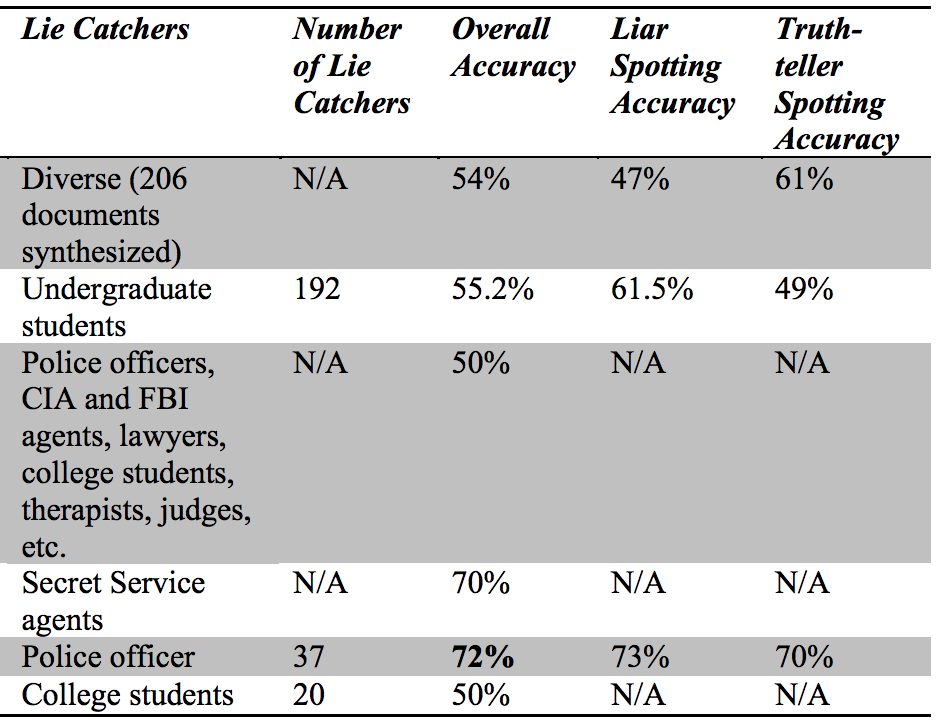
\includegraphics[width=0.75\textwidth]{Ppl_lie_accuracy}
	\caption{Performance on deceit detection by human observers \cite{SU201652}.}
\end{figure}
 
\clearpage

% also talk about non-contact
\section{State of the Art} \label{sota}
How are lies detected? At the moment there are a lot of different instruments and technologies to attempt to detect deceit, ranging from analyzing psychological features, to using the polygraph or thermal cameras and machine learning approaches.

In computer vision specifically, lie detection is a somewhat new field of research, and as such it's done using many different techniques, employing not only RGB cameras but also physical sensors and thermal cameras and using voice, gaze, action and body analysis tools, all of this often aided by machine learning techniques, and by combining many of these modalities together to achieve better results.

We now proceed to describe the state of the art, based on the latest researches done in the field, with specific focus on computer vision:

\subsection{Speech}
Speech is one of the many methods that can be used to recognize if a person is lying. In fact, the speech signal contains linguistic, expressive, organic and biological data \cite{norena}.

One of the most used indicator of deception in various studies has been the response latency \cite{EaseLying}, since inventing a lie requires additional cognitive load as opposed to remembering the truth. The authors also notice that habitual lying makes it easier, and conversely often being spontaneous and telling the truth makes lying harder.\\
Another indicator of lying is the speech rate, especially when it's different from the average rate of a specific person \cite{TemporalCues}. Other verbal cues like grammar usage and word frequency have been used and have achieved high accuracy in psychological researches \cite{PorterTruthLying}.

Speech analysis can reveal changes that affect behavior, such as stress, emotion, deception etc. by analyzing the pitch and the stress level. When a stressful situation arises, the hormonal levels of the body change, and this causes an increase in blood pressure and heart rate. This in turn affects the muscle in the respiratory system, and so speech is affected \cite{norena}.

In sound processing, the mel-frequency cepstrum (MFC, Fig. \ref{fig:MFCC}) is a representation of the short-term power spectrum of a sound. Mel-frequency cepstral coefficients (MFCCs) are coefficients that collectively make up the MFC \cite{wiki:mfcc}.

\begin{figure}[H]
	\centering
	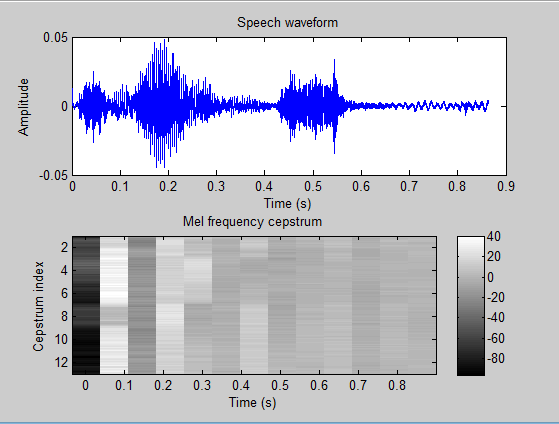
\includegraphics[width=0.5\textwidth]{MFCC}
	\caption{Topside is the spoken word, bottom is the MFCC derived from the word}
	\label{fig:MFCC}
\end{figure}

In \cite{relidss} the authors created a new database by making 40 candidates try to deceive them while telling truthful or deceptive statements for about one to two minutes each. From this experiment they extracted MFCC and pitch, so that they could process them through Matlab's Voice Box. \\
After acquiring the data, an SVM classifier was trained to classify new data, obtaining an accuracy of Lie and Truth detection from speech audio respectively of 88.23\% and 84.52\%.

In \cite{Mihalcea:2013:ADD:2522848.2522888} Perez et al. utilize a dataset of 140 videos created by users who uploaded either truthful or deceptive statements. They collected the transcriptions from the videos both manually and via automatic speech recognition software. By using a bag-of-words representation of the transcripts they build a vocabulary, and to classify the data they employ a SVM and Naive Bayes classifier, achieving 73\% accuracy.

\clearpage
 
\subsection{Eyes}
Using the eyes to detect lies is one of the most studied approaches, as the eyes hold a significant amount of information regarding our thinking and emotional state \cite{FUKUDA2001239} (Fig \ref{fig:eye-lies}). We will focus our description on the Computer Vision approaches.

% TODO: this pic has nothing to do with what is written here
\begin{figure}[H]
	\centering
	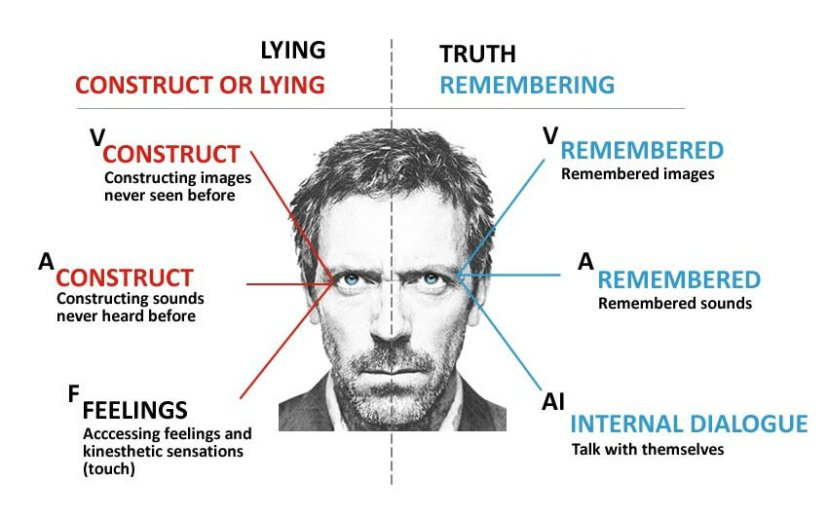
\includegraphics[width=0.85\textwidth]{eye-lies}
	\caption{Eyes could hold a lot of informations regarding what we are thinking \cite{eyeLies}.}
	\label{fig:eye-lies}
\end{figure}

An important advantage of using the eyes as a vehicle for deception detection is that it is possible to generate a non invasive approach while analyzing the eyes, meaning that subjects do not need to willingly participate or even know if they are being examined or not (the moral matter should be considered in another setting), and there could be no need to have huge and expensive machinery, like for example the polygraph or a fMRI machine.

Cognitive load, which is set to increase while lying, is one of the most significant factor for deception detection and can be analyzed through the eyes. Important are also the blink rate, gaze aversion and pupil dilation.

In \cite{8125844} the authors utilize high speed cameras to record and analyze blink count and blink duration of 50 subjects while asking 10 control questions, to see if there is a variation in them while the subject is being questioned. The authors analyzed the resulting images frame by frame and based on the facial landmarks around the eye they recognize AU45, the action unit for blinking. The results shows that both blink duration and count are increased while lying.

In another study, Leal and Vrij \cite{Leal2008} asked 26 people, 13 liars and 13 truth tellers, to lie or tell the truth in a target period, while having a baseline from two preceding periods. The eye blinks during the target and baseline periods and directly after the target period (target offset period) were recorded.\\
Compared to the baseline periods, lying subjects show a decrease in eye blinks during the target period and an increase in eye blinks during the target offset period. This means that there is a decrease in eye blinks while lying and an increase just after lying. This pattern resulted very different for truth tellers, showing that there is a significant difference in eye blink behavior between truthfulness and deception.

Singh et al. in \cite{7324092} show that while lying there is an increase in cognitive load and a significant decrease in eye blinks, directly followed by an increase in blink rate as soon as the cognitive demand ceases, after telling the lie. A threshold is set by the authors for this study, either at 26 blinks per minute or it is calculated personally using the average blink rate from a blink detection algorithm. Blink detection is done through MATLAB using the HAAR Cascade algorithm.

Lim et al. study eye gaze \cite{Lim:2013:LTE:2535948.2535954} to investigate the relation with lie detection. The result supports the theory that an increase in cognitive load leads to a decrement in the number of eye movements while lying.

Bhaskaran et al. measure deception by the deviation from normal behavior at critical points during an investigative interrogation \cite{5771407} . For starters, a dynamic Bayesian model of the eye movement is trained during a normal conversation with each of the 40 subjects of the experiment. \\
The remainder of the conversation is then broken into pieces and each piece is tested against the normal behavior. The deviation from normality are observed during critical points in the interrogation and used to deduce the presence of deceit, obtaining an accuracy of 82.5\%.

In \cite{7165946} Proudfoot et al., using latent growth curve modeling, research how the pupil diameter changes over the course of an interaction with a deception detection system. The assumption is that anxiety changes the pupil diameter. The subjects are presented with crime-relevant target items (possibly incriminating) and non relevant items. \\
The results indicate that the trends in the changes are indicative of deception during the interaction: pupil diameter is initially bigger for guilty subjects relative to innocent ones. Also the pupil diameter of the participants decreased between subsequent sections of the test, specifically the magnitude of the decrease was greater for guilty subjects who did not see incriminating items.

\subsection{Neuroscience}
Electroencephalogram (EEG) and functional Magnetic Resonance Imaging (fMRI) have been employed for lie detection with good results for a long time, but at the cost of invasiveness, since both methods require big machinery, a suitable environment, and a subject willing to participate.

EEG is a monitoring method that records brain activities based on its potential.

In \cite{7440177} Simbolon et al, use Event Related Potentials (ERP) to measure brain response directly from thought or perception. Among the many types of signals that constitute the ERP signal, P300 (Fig. \ref{fig:EEG}) is the most critical for lie detection, as it appears as a response to meaningful rare stimuli (called odd ball stimuli). \\
Eleven males of age between 20 and 27 took part in the study. The gathered data were then divided into training and test sets to produce different models. The highest accuracy of 70.83\% was reached by a SVM classifier in detecting lying subjects.

\begin{figure}[H]
	\centering
	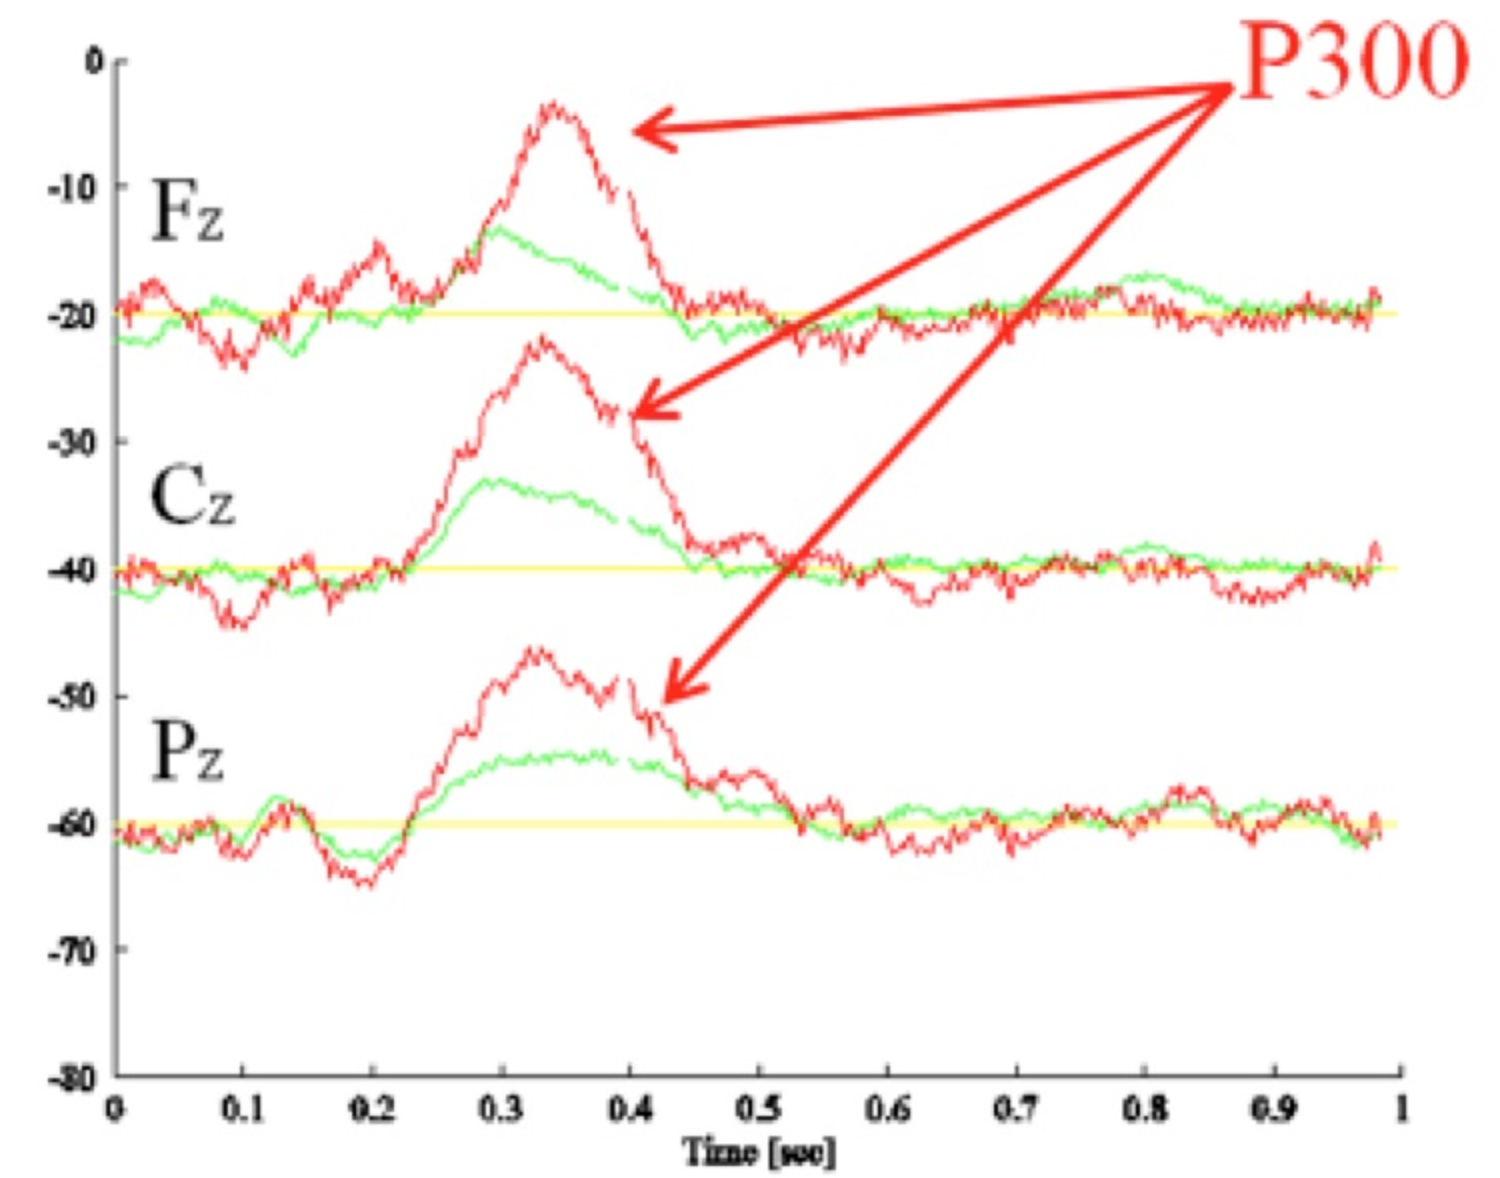
\includegraphics[width=0.75\textwidth]{EEG}
	\caption{EEG of P300 waves image on channels Fz, Cz, and Pz}
	\label{fig:EEG}
\end{figure}

In \cite{Lai2017} twenty people of ages between 22 and 24 years old were subject to a card test using an EEG machine. EEG signals were collected using electrodes attached to the subject’s head. The authors used the EEG signals to identify useful frequency bands and to measure lying state based on spectral analysis, with the use of fuzzy reasoning, obtaining 89.5\% detection accuracy.

Arasteh et al. \cite{7511728} utilize an alternative approach to the polygraph, the P300 Guilty Knowledge Test (GTK). GTK is based on the amplitude of P300 ERP wave as an index for the subject's recognition of concealed information. The Guilty Knowledge Test works on the assumption that among many similar unfamiliar topics, the recognition of familiar ones will be followed by a different response. \\
62 subjects were part of this experiment and participated in a mock crime followed by the P300 GTK. The authors used empirical mode decomposition (EMD) to extract features from the EEG signal and modeled them trough matlab. A genetic algorithm was then utilized for the feature selection and to handle the dimensionality increase of this approach. The classification accuracy of guilty and innocent subjects was 92.73\%.

Another neuro-scientific approach to lie detection is functional Magnetic Resonance Imaging (fMRI). fMRI measures brain activity by detecting changes associated with blood flow (Fig. \ref{fig:fMRI}). This technique relies on the fact that cerebral blood flow and neuronal activation are coupled. When an area of the brain is in use, blood flow to that region also increases \cite{WikifMRI}.

In most of the experiments with fMRI and lie detection, candidates are instructed to lie and tell the truth in specific situations, and the brain activity from these instances is compared to a baseline condition. The regions showing greater activation for lies than truth are supposed to be the most significant for deception detection. In a recent study it is shown that there is considerable agreement on the significant areas of the brain that regard lying \cite{fMRILD}.

\begin{figure}[H]
	\centering
	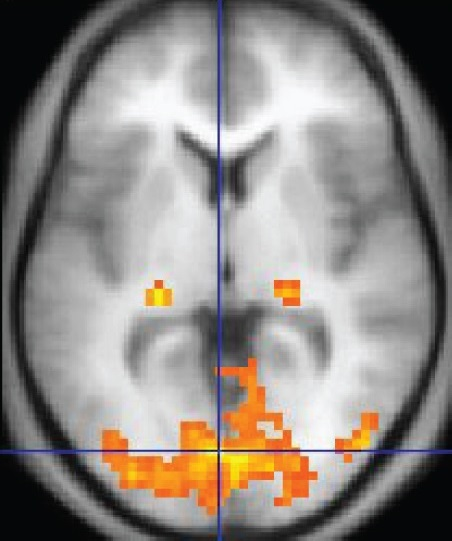
\includegraphics[width=0.55\textwidth]{fMRI}
	\caption{fMRI image with yellow areas showing increased activity compared with a control condition  \cite{WikifMRI}}
	\label{fig:fMRI}
\end{figure}

As much as fMRI is useful for lie detection, it presents some shortcomings \cite{fMRIDD} \cite{fMRIDA}: many fMRI studies are small, not replicated and done with just a few subjects; there are some contradicting results between some studies; most of the studies are not done in a contest of high stake deception, but in a controlled environment where subjects are asked to lie about some topic or event, but often without a real interest in being deceitful. Another important point is that the fMRI approach requires collaboration and expensive equipment to be carried out, so this is a very limiting factor.

\subsection{Thermal Imaging}
In thermal imaging, thermal features are extracted from the face using a high definition thermal camera. The objective is to analyze what kind of differences occur when a subject responds truthfully or deceptively to particular stimuli.

\begin{figure}[H]
	\centering
	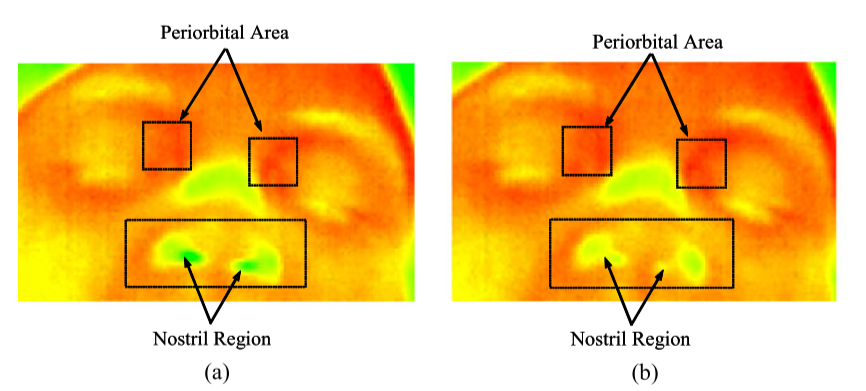
\includegraphics[width=1\textwidth]{thermal}
	\caption{Examples of thermal images during (a) questioning and (b) answering \cite{6967765}}
\end{figure}

According to a recent study \cite{Abouelenien:2015:TAD:2823465.2823470} examining 30 subjects, the most relevant zones for deception detection, seen by utilizing thermal equipment, and located in the facial area are the forehead and periorbital regions. \\
In this study the subjects were registered with a thermal camera for one minute to extract the baseline features, and after that the interviewers asked a series of questions. A thermal map was created from the registrations using the Hue Saturation Value to differentiate between lies and truths.

In \cite{Rajoub} the authors set up an experiment to collect 492 responses from 25 participants, using a deception scenario requiring the subjects to learn a story, provided by the authors, and practice their stories before hand by giving them sample questions, so that the cognitive load would increase when receiving new and unseen questions during the interview.

At the beginning of the interview four baseline questions were asked to register the initial thermal state of the subjects, and then a series of questions were asked, with answers both present and missing from the provided story. After extracting the periorbital region's thermal variation, a k-nearest neighbor classifier was used, with an 87\% accuracy in predicting lies or truths.

In \cite{6967765} data are gathered non-intrusively from the nostril and periorbital regions using two dimensional far infrared cameras. The study lasted for two years and covered 18 tests subjects involved in real crime cases. The temperature is extracted and converted in change in blood flow velocity, and a signature of the respiration pattern is determined in terms of the ratio of the measured maximum and minimum temperatures in the nostril area. The classification rate for this study is 88.5\%.

\subsection{Multimodal}
After seeing all these different techniques to detect lies, it's only natural for researchers to try and fuse or aggregate some of them to see if it's possible to achieve better results \cite{Abouelenien:2014:DDU:2663204.2663229}.

In \cite{Abouelenien:2016:ATV:2910674.2910682} Abouelenien et al. collect data from a dataset of 30 subjects to examine thermal and visual clues of deception. Their aim is to identify the regions that offer higher capability of detecting deceit. \\
The method employed uses the CERT (Computer Expression Recognition Toolbox) to detect facial expression and encodes them through Action Units, a way to codify almost any kind of muscle movements on the face. \\
To extract thermal features they create a thermal map using gray-scale and Hue Saturation Value. They also calculated normalized blinking rates and the mean head orientation angle along the entire length of the response. In addiction over 60 physiological features are extracted and stored with the use of sensors and other RGB cameras. The experimental results show that the non-contact feature fusion model outperforms traditional physiological measurements, and that the forehead region is one of the most promising areas to gather information for deception detection using thermal imaging.

In a following paper \cite{7782429} Abouelenien et al. explore a multimodal deception detection approach comprised of physiological, linguistic, and thermal features on a new dataset of 149 recordings. They set out to determine which is the most discriminative region of the face to differentiate between truth and lies based on thermal imaging, and perform feature analysis using a decision tree model. The results show that the forehead could be a better indicator of deceit than the periorbital area. The physiological features did not contribute very much, while the linguistic feature played a critical role, where self-referencing and exaggeration words where big indicators of deceit. The overall accuracy of the system is ~70\%.

Another example of multimodal detection is found in \cite{DBLP:journals/corr/abs-1712-04415} where Wu et al. develop a framework to automatically detect deception in videos of trials. They utilize three modalities: vision, audio and text. For vision, they employ various classifiers trained on low level video features to predict human micro-expressions, and to successively predict deception. Interestingly, IDT (Improved Dense Trajectory) features, often used to recognize actions in videos, are good predictors of deceptive behavior. \\
The authors decided to fuse the score of the classifiers on IDT and micro-expressions to boost the performance. Regarding text, the transcript of the considered videos are analyzed, but the performance increase is very marginal. \\
For speech, they integrated the vision side with Mel Frequency Cepstral Coefficient (MFCC) features analysis from the audio, boosting the performances significantly, reaching an AUC of 0.877. 

Noje et al. \cite{7367432} set up a study with ten subjects to observe the potential of head movements in lie detection. They built an application to detect head movement and position by performing a frame to frame analysis on a video stream. A correlation was made between head movement/position and the identification of lies. The results of the study are not concluding as this data can't be utilized without being incorporated with other modalities such as voice, gaze, words, expressions et cetera.

In \cite{Perez-Rosas:2015:DDU:2818346.2820758} Perez et al. utilize real life trial videos to identify deception, employing a model that extracts features from both linguistic and gesture modalities. The verbal features consist of unigrams and bigrams derived from the bag-of-words representation of the video transcripts, while gesture features are taken from the annotations performed using the MUMIN coding scheme, where each feature indicates the presence of a gesture only if it's present in the majority of the video. Using Decision Trees and Random Forest classifiers they achieve between 60\% and 75\% accuracy.

\begin{figure}[H]
	\centering
	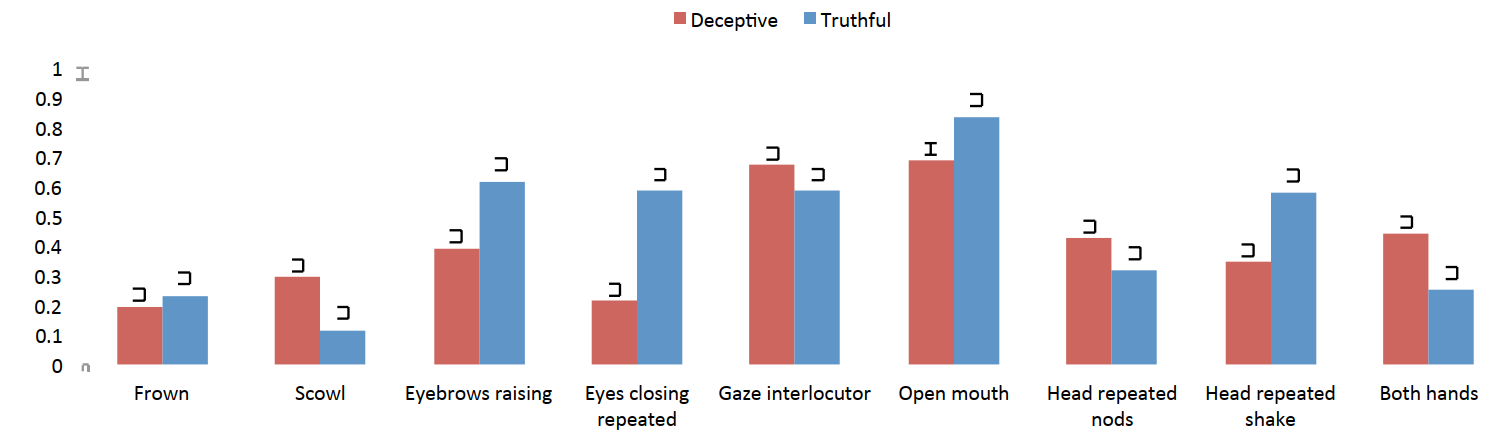
\includegraphics[width=0.9\textwidth]{non_verbal_perez}
	\caption{Distribution of non-verbal features for deceptive and truthful groups \cite{Perez-Rosas:2015:DDU:2818346.2820758}.}
\end{figure}

\subsection{Facial Expression and Micro-Expressions}
Facial Expressions are one of the main methods that we use to express our emotions, and are developed since the first months of our life to help us communicate our feelings to others. But what happens when we want to hide our emotions instead? 

Facial micro-expressions are very fast (1/2 to 1/25 of a second) and involuntary expressions that come up on the human face when we are trying to suppress or hide an emotion, and are very difficult to control using just one's willpower \cite{EkmanER}.

\begin{figure}[H]
	\centering
	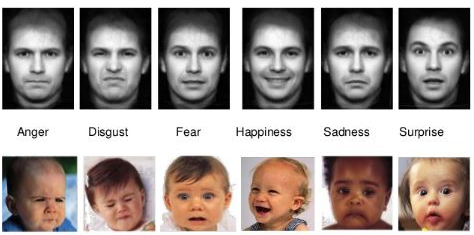
\includegraphics[width=1\textwidth]{expr}
	\caption{Six basic Facial Expressions in adults and children \cite{baby_fe}.}
\end{figure}

Studying and classifying micro-expression is very valuable and has many applications, especially in psychology and forensic sciences, but it is a hard feat as the duration is very short and the intensity is low.\\ 
Micro-expressions have been studied since 1966 to recognize and distinguish real or fake emotions, initially by Haggard and Isaacs \cite{Haggard}, and three years later by Ekman and Frisen \cite{EkmanLeakage}.

Substantial work on Micro-Expressions has been done by Pfister, Li et al. In \cite{pfister2011micro} they collaborated with psychologists to design an induced emotion suppression experiment. The data was collected with a high speed camera to be able to register the micro expressions of the subjects. A Temporal interpolation model was used to counter the shortness of the video length, while multiple kernel learning, random forest and SVM were used to classify micro expressions reaching an accuracy of 71.4\%.

The lack of a big and well formed database was one of the biggest hindrance to their research. To solve this problem in \cite{xli2012spontaneous} they reveal a new dataset, the Spontaneous Micro-expression Database (SMIC), which includes 164 micro-expression video clips taken from a group of 20 participants.\\
They used two high speed cameras to record the face of the subjects while they were watching a selection of videos that induced strong emotional response, and they had to try and suppress those emotions. After the video the subjects had to answer about the emotions they felt while watching it. The data were then segmented and labeled by two annotators.

A study of spontaneous micro expression spotting and recognition methods was done in \cite{xli2015reading}. A new training-free method, based on feature difference contrast for recognizing micro-expressions was presented. The features are extracted from the video using Local Binary Pattern (LBP) and Histogram of Optical Flow. \\
To recognize the Micro expressions, the authors performed face alignment and temporal interpolation, then trained an SVM classifier. \\
This micro-expression framework was tested on the SMIC and CASMEII database with very good results. After combining micro-expressions spotting and recognition they released a new micro-expression analysis system (MESR) that is able to recognize micro-expressions from spontaneous video data.

Owayjan et al. \cite{6462897} designed a lie detection system using micro-expressions. At first an embedded video system is used to record the subject interview. The video stream is converted into frames, and each frame is processed in four stages: converting the images, filtering out useless features, applying geometric templates and finally extracting the measurements to detect the micro-expressions. \\
Results show that up to eight facial expressions can be recognized, and that lies can be discerned with high precision.

In \cite{10.1007/978-3-319-47955-2_27} Kawulok et al. explore how to exploit fast smile intensity detectors to extract temporal features using a SVM classifier. Using exclusively a face detector, without localizing or tracking facial landmarks, they analyze the smile intensity time series. They then employ an SVM classifier to improve training from weakly labeled datasets. Then, to train the smile detectors, they use uniform local binary pattern features. This allows to detect, in real time, between spontaneous or posed expressions.

Su et al. \cite{SU201652} aim to test the validity of facial clues to deception detection in high-stakes situations using computer vision approaches. By using invariant 2D features from nine separate regions of the face they perform facial analysis on eye blink, eyebrow motion, wrinkle occurrence and mouth motion, integrated with a facial behavior pattern vector. Training a Random Forest to classify the patterns into deceptive or truthful, they achieved a 76.92\% accuracy.

\subsection{Action Units} \label{au}
Action Units (AUs) are defined as a contraction or relaxation of one or more muscles. They have been used in the Facial Action Coding System (FACS), a system developed initially by Hjorztsjö \cite{facsCH} and then improved by Freisen and Ekman \cite{facs1978}, that categorizes all the facial movements by their appearance on the face.

Using FACS it's possible to code nearly any facial expression by deconstructing them into Action Units. For example the Duchenne smile (felt smile) is a combination of AU6 (orbicularis oculi, pars lateralis) and AU12 (zygomatic mayor) as we can see from fig. \ref{fig:duchenne}.

\begin{figure}[H]
	\centering
	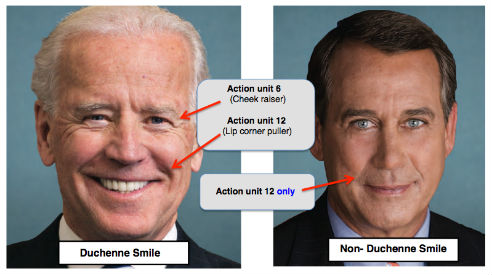
\includegraphics[width=1\textwidth]{duchenne}
	\caption{Duchenne smile (real) vs non Duchenne (fake).}
	\label{fig:duchenne}
\end{figure}

In the FACS there are 44 AUs categorized with five level of intensity (A to E). Most of the AUs have an onset, peak and offset phase, as shown in fig. \ref{fig:au_intensity}. 

\begin{figure}[H]
	\centering
	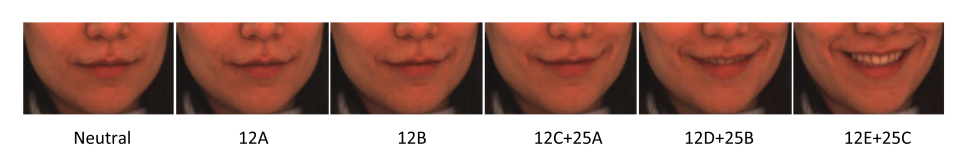
\includegraphics[width=1\textwidth]{au_intensity}
	\caption{Facial images with AU intensity variations (AU12: lip corner puller, AU25: lips part) \cite{DISFA}.}
	\label{fig:au_intensity}
\end{figure}

By using AUs is possible to recognize emotions based on the combination of AUs displayed (Fig. \ref{fig:AUs}).

\begin{figure}[H]
	\centering
	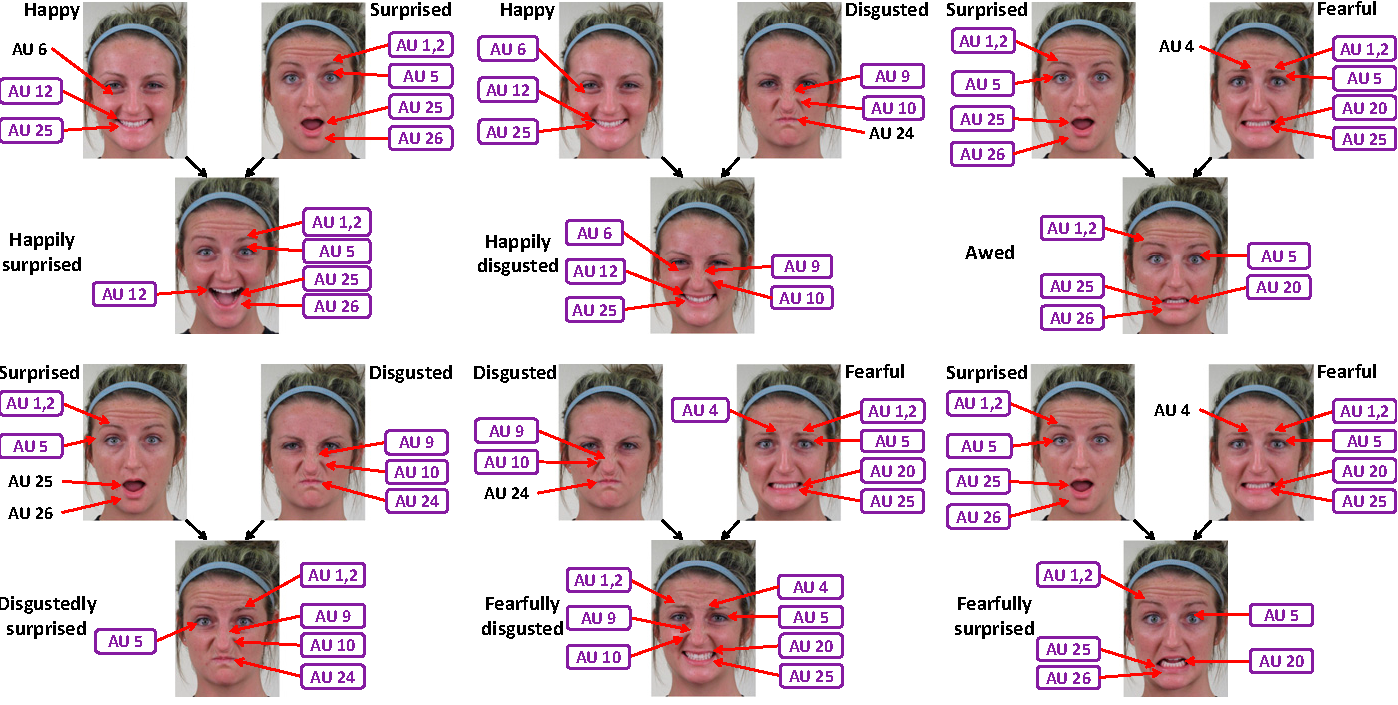
\includegraphics[width=1\textwidth]{AUs}
	\caption{AUs of six compound facial expressions of emotion. The AUs of the basic emotions are combined to produce the compound category \cite{Du2014CompoundFE}.}
	\label{fig:AUs}
\end{figure}

Substantial work on AU classification and intensity estimation has been done in \cite{Baltru2015} by Baltrusaitis et al. while developing the OpenFace \cite{Baltru2016} system. \\
Baltrusaitis et al. developed a real-time Facial Action Unit occurrence and intensity detection system based on appearance and geometric features, using Histogram of Oriented Gradients, Shape Parameters and Landmark Locations. They achieved good results by using a median based feature normalization technique so that they could account for person specific neutral expressions.

In \cite{HaoWangAU} Hao et al. explore the dependencies between AUs, and propose a new AU recognition method consisting of a three layer Bayesian network where the top two layers are latent regression Bayesian networks (LRBN). \\
LRBN are graphical models consisting of a visible layer representing the ground truth for AUs and a latent one. LRBN is able to capture the dependencies between AUs. They tested this system on the CK+ \cite{CK+}, SEMAINE \cite{SEMAINE} and BP4D \cite{BP4D-Spontaneous} database, demonstrating that their approach can accurately capture AU relationships.

In \cite{AU_LSTM} the authors try to model three fundamental aspects of automated AU detection: spatial representation, temporal modeling, and AU correlation. They proposed an approach using a hybrid network architecture. \\
Spatial representation is extrapolated by using a Convolutional Neural Network (CNN). For temporal dependencies Long Short-Term Memory Neural Networks (LSTM) are stacked on top of the CNN. \\
The output of LSTMs and CNNs are then fused together to predict 12 AUs on a frame to frame basis. This network was then tested on the GFT and BP4D \cite{BP4D-Spontaneous} dataset, gaining improvements over standard CNN.

De la Torre et al. \cite{AU_STM} \cite{AU_STM2} tackle this problem by personalizing a generic classifier without requiring additional labels for the test subject (unsupervised). They use a transductive learning method, referred as Selective Transfer Machine (STM), that personalizes a generic classifier by attenuating people specific biases. This is done by  learning a classifier and re-weighting the training samples most relevant to the subject. \\
The performance of STM were compared to generic classifiers and cross-domain learning methods and evaluated on CK+ \cite{CK+}, GEMEP-FERA, RUFACS and GFT dataset, and STM is shown to outperform the generic classifiers on all datasets.

Although there has been a lot of progress during the years, there is still a lot of work to be done regarding AUs, since many approaches to automatic facial AU detection fail to account for individual difference in morphology and behavior for the target person. This is a hard problem because it's difficult for classifiers to generalize to very different subjects, and training a person-specific classifier is neither feasible (very low training data) nor has particular theoretical interest. 

\clearpage

\section{Contributions and Outline} \label{contrib}

\subsection{Contribution}
The human face holds many clues to recognize emotions and to discern truth and lies. Human emotions can be recognized mainly by the expressions we make when a situation arises, such as being scared or happy. Those expressions are translated into movements of the muscles of the face. Building on this idea, the objective of this thesis is to classify if a person is lying or telling the truth based on the action units (muscular movements of the face) extracted from a video. 

It is important to note that all the videos are taken from high stakes situations, specifically court trials, so that all the liars and truth tellers have a big incentive in lying or telling the truth, since the validity of many studies is questionable based on the fact that the emotions analyzed are posed (non spontaneous). 

As far as we know this is the first time a study uses an SVM to classify between truth and lies in high stakes situations, using extracted action units.

\subsection{Outline}
This thesis is composed by the following chapters:

\begin{itemize}
	\item \textbf{Chapter 2} is about Machine Learning. We will talk about classification, regression, supervised learning and some techniques such as Random Forest and SVM.
	\item \textbf{Chapter 3} will describe the architecture of our work, explaining landmark detection, action unit intensity and presence estimation, and the process to discriminate between deception and honesty.
	\item In \textbf{chapter 4} we discuss the dataset and explain the experimental procedure of training and testing a binary classifier for discerning truth and lies.
	\item \textbf{Chapter 5} is where we discuss the results of this work.
	\item In \textbf{chapter 6} we draw the conclusions, and future work is presented. 
\end{itemize}


\chapter{Architecture}
%todo: complete, this is what my program does
In this chapter we will discuss the architecture of our framework and the tools used for this thesis in Deception Detection. We will first explain the general architecture to perform deception detection, then we will introduce the OpenFace toolkit (\ref{OpenFace}), and describe landmark detection (\ref{landmark_det}), action unit recognition (\ref{au_det}) and the deception detection process (\ref{dec_det}).

\section{General Architecture}
%todo with images + change title
The general idea of this thesis is to classify whether a person is telling the truth or lying, by analyzing the subject's facial movement, extracted using an RGB camera, during a video. To achieve this it is fundamental that the subject's face results visible during the videos.

We implemented this idea using a Support Vector Machine classifier. 

The architecture utilized is shown in fig \ref{fig:architecture} and is composed this way:

\begin{itemize}
	\item We gather a video of a person in a high stake situation.
	\item Detect the face of the person in the video using Constrained Local Neural Field.
	\item Detect the facial landmarks using Convolutional Experts Network.
	\item Extract the appearance features in the form of Histogram of Oriented Gradients and perform dimensionality reduction and feature normalization through Principal Component Analysis.
	\item Extract action unit presence and intensity from the videos using a SVM.
	\item Feed the extracted data to train an SVM for classification on a test set.
\end{itemize}

\clearpage

\section{OpenFace} \label{OpenFace}
The OpenFace \cite{Baltru2018} toolkit is a tool for machine learning and computer vision researchers, created by Baltrusaitis et al., to support performing facial landmark detection, head pose estimation, action unit recognition, feature extraction and eye gaze estimation. 

\begin{figure}[H]
	\centering
	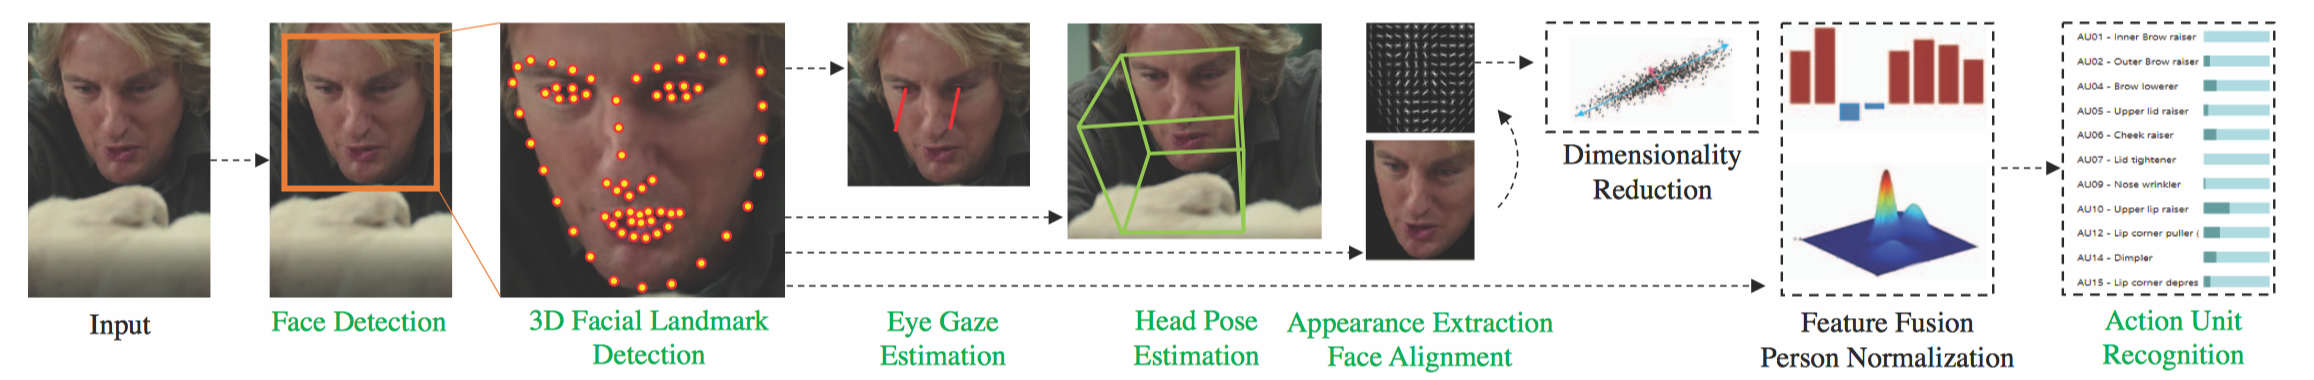
\includegraphics[width=1\textwidth]{openface20_pipeline}
	\caption{OpenFace Pipeline \cite{Baltru2018}}
	\label{fig:openface20_pipeline}
\end{figure}

%TODO: check this new addition
This tool is customizable in the way that all the SVM models and neural networks can be trained with new datasets, and the code is open source, so it can be changed to fit the needs of the experimenters.

%TODO: expand saying "we now describe how we used this tool for x y z...?


\clearpage

\section{Landmark Detection} \label{landmark_det}

The first step in Action Unit identification is to detect the facial landmarks. To accomplish this a local detector called Convolutional Experts Network (CEN) (Fig. \ref{fig:CEN}) is utilized. 

CEN has the advantage of aggregating a neural architecture and patch experts which are local detectors and are used to evaluate the probability of a landmark being aligned at a particular pixel location. CEN can learn different patch experts and adapt to diverse appearance models without explicitly labeling attributes.

\begin{figure}[H]
	\centering
	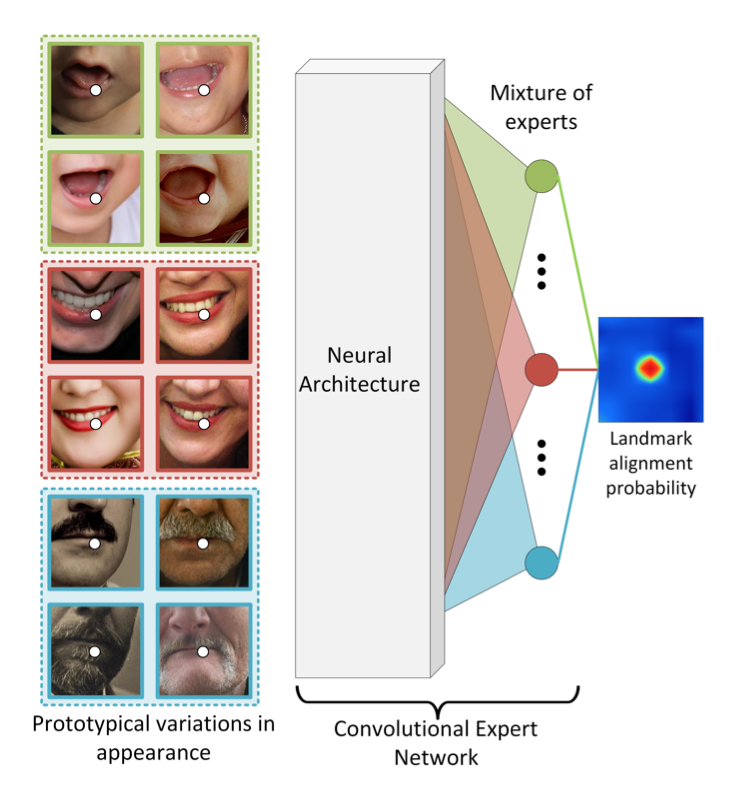
\includegraphics[width=0.75\textwidth]{CEN}
	\caption{Facial landmarks naturally cluster around appearance prototypes (facial hair, expressions, make-up etc). To model such appearance variations a Convolutional Experts Network is used to merge the advantages of neural architectures and mixtures of patch experts, to model landmark alignment probability \cite{Baltru2017}.}
	\label{fig:CEN}
\end{figure}

%TODO: write better?
OpenFace uses a Convolutional Experts Constrained Local Model (CE-CLM) \cite{Baltru2017}, which is a Constrained Local Model (CLM) that uses CEN as a local detector. 

A Constrained Local Model is class of methods for locating sets of points (constrained by a statistical shape model) on a target image \cite{clm_cootes}.

Generally the procedure is as follows (Fig. \ref{fig:CLM}):
\begin{itemize}[noitemsep]
	\item Sample a region from the image around the current estimate, projecting it into a reference frame.
	\item For each point, generate a "response image" giving a cost for having the point at each pixel.
	\item Search for a combination of points which optimizes the total cost, by manipulating the shape model parameters.
\end{itemize}

%todo: pic from https://pdfs.semanticscholar.org/c2a3/850becae2799b0e591e7ab1008b84897d6e9.pdf
\begin{figure}[H]
	\centering
	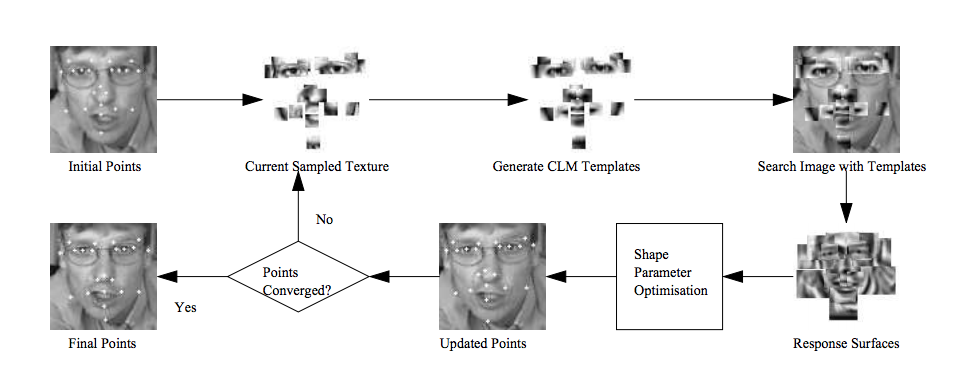
\includegraphics[width=1\textwidth]{CLM}
	\caption{Overview of CLM \cite{clm_cootes}.}
	\label{fig:CLM}
\end{figure}

CLM are used to model the appearance of each facial landmark individually by using local detectors and a shape model for constrained optimization. 

The CE-CLM is divided in two fundamental parts: response map computation using CEN, and shape parameter update.

In the first step, the landmarks alignment is computed separately from the other landmarks. \\
In the second phase, all landmarks are considered together and for misaligned landmarks and irregular shapes their position is penalized, using a Point Distribution Model (PDM).

\subsection{CEN}
In the initial step, the objective is to generate a response map to localize the individual landmarks. This is performed by assessing the landmark alignment probability at specific pixel locations. \\
CEN takes in input a Region of Interest (ROI) around the currently estimated position of a landmark, and outputs a response map that calculates the landmark alignment probability at each pixel location (Fig. \ref{fig:landmark_det}).

\begin{figure}[H]
	\centering
	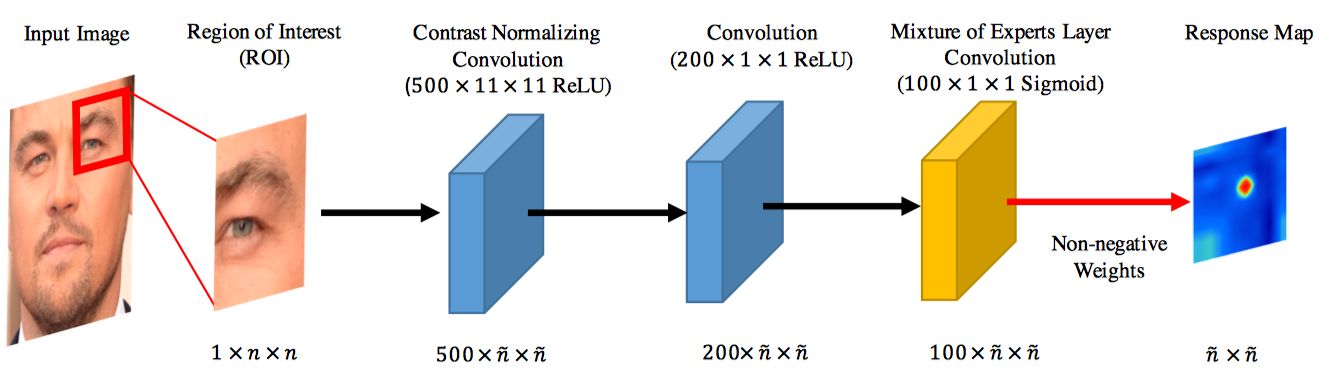
\includegraphics[width=1\textwidth]{landmark_det}
	\caption{Overview of the Convolutional Experts Network model. The output response map is a non-negative and non-linear combination of neurons in ME-layer using a sigmoid activation \cite{Baltru2017}.}
	\label{fig:landmark_det}
\end{figure}

In order to do all this, the ROI is initially passed in a Contrast Normalizing Convolution layer to perform z-score normalization and to calculate the correlation between input and kernel. The output is then convolved in another layer of ReLU neurons (convolution is an operation on two functions to produce a third function that expresses how the shape of one is modified by the other).

The last neural layer before the response map is the Mixture of Expert Layer (ME-layer), and it can model the alignment probability using a combination of patch experts (local detectors) that are able to represent different landmarks appearance prototypes by outputting individual votes on alignment through a sigmoid function. The response maps from all the local detectors are then combined in the last layer, giving the final alignment probability.

\subsection{Point Distribution Model}
%TODO: from wiki modify a bit
The Point Distribution Model is a used to represent the mean geometry of a shape and some statistical modes of geometric variation inferred from a training set of shapes \cite{wiki:PDM}. 

\begin{figure}[H]
	\centering
	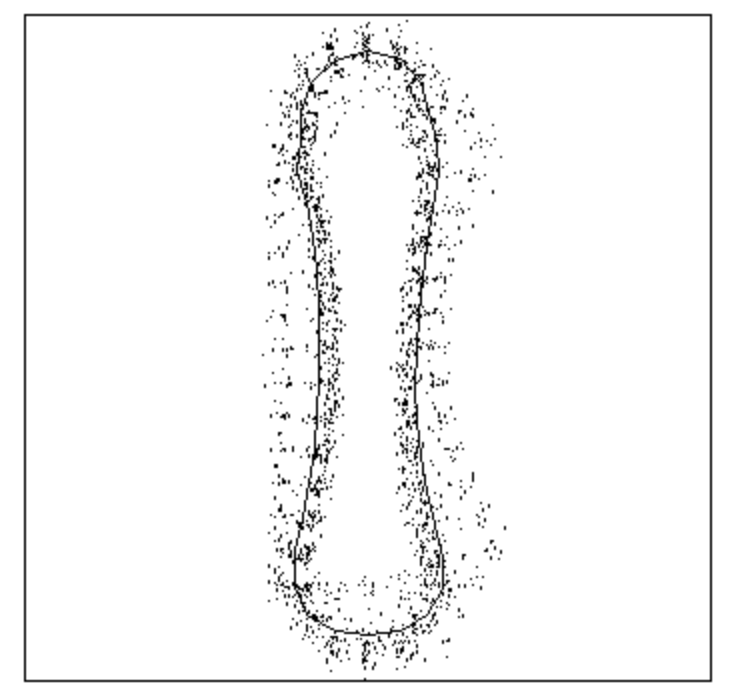
\includegraphics[width=0.45\textwidth]{PDM}
	\caption{PDM of a metacarpal. Dots mark the possible position of landmarks, and the line denote the mean shape \cite{PDM}.}
	\label{fig:PDM}
\end{figure}

Point distribution models rely on landmark points. The general PDM works this way:
\begin{enumerate}
	\item A set of training images are manually landmarked to sufficiently approximate the geometry of the original shapes. 
	\item This \textit{k} landmarks are aligned in two dimensions resulting in \\
	$\mathbf{X} = (x_1,y_1, \dots, x_k, y_k)$
	\item The shape outlines are reduced to sequences of k landmarks, so that any given training shape can be defined by the vector $\mathbf{X} \in {\mathbb{R} ^{2k}}$.
	\item The matrix of the top $d$ eigenvectors is given as $\mathbf{P} \in \mathbb{R}^{2k \times d}$, and each eigenvector describes a principal mode of variation along the set.
	\item A linear combination of the eigenvectors is used to define a new shape $ \mathbf{X} '$, mathematically defined as: 
	\begin{equation}
	\mathbf {X}' = {\overline {\mathbf {X}} + \mathbf{P} \mathbf{b}}
	\end{equation}
	
	where $ {\overline {\mathbf {X}}}$ is defined as the mean shape across all training images, and $\mathbf {b}$ is a vector of scaling values for each principal component. 
	\item By modifying the variable $\mathbf {b}$  an infinite number of shapes can be defined. $\mathbf {b}$ shouldn't generally be modified more than $\pm3\sigma$ \cite{wiki:PDM}.
\end{enumerate}

With the OpenFace framework Point Distribution Model \cite{PDM_RLMS} we model the location of facial feature points in the image, using non-rigid shape and rigid global transformation parameters.

The application of PDM has two objectives:

\begin{itemize}
	\item They are employed to control the landmark locations.
	\item They are used to regularize the shapes in the CE-CLM framework by using Non-Uniform Regularized Landmark Mean Shift (NU-RLMS) \cite{Baltru2013}.
\end{itemize}
This has an effect in the final detected landmarks, where the irregular shapes are imposed a penalty.

The results can be seen in the figure \ref{fig:land_det_ex} below for different images with different illuminations and angles. 

\begin{figure}[H]
	\centering
	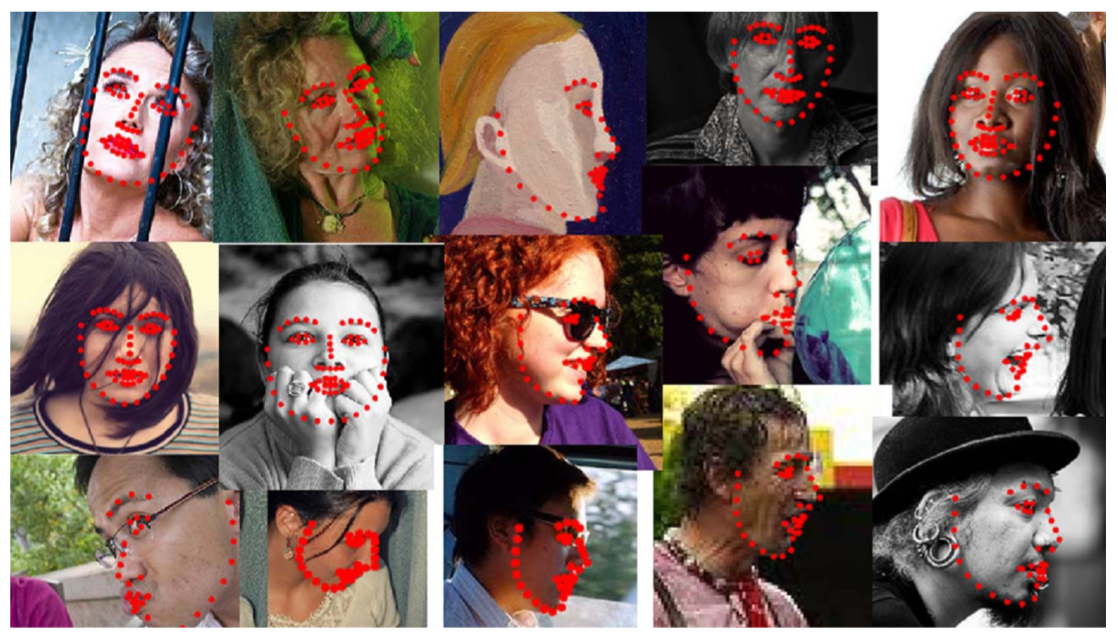
\includegraphics[width=0.85\textwidth]{land_det_ex}
	\caption{Example of different facial landmarks detected in diverse conditions and viewing angles. \cite{Baltru2018}.}
	\label{fig:land_det_ex}
\end{figure}

\clearpage

\section{Action Unit Detection} \label{au_det}
Action Unit (AU) detection plays a fundamental role in our work. We now describe the process used to detect the AUs through an SVM, starting with an overview of the datasets utilized for training the SVM in AUs detection.

\begin{figure}[H]
	\centering
	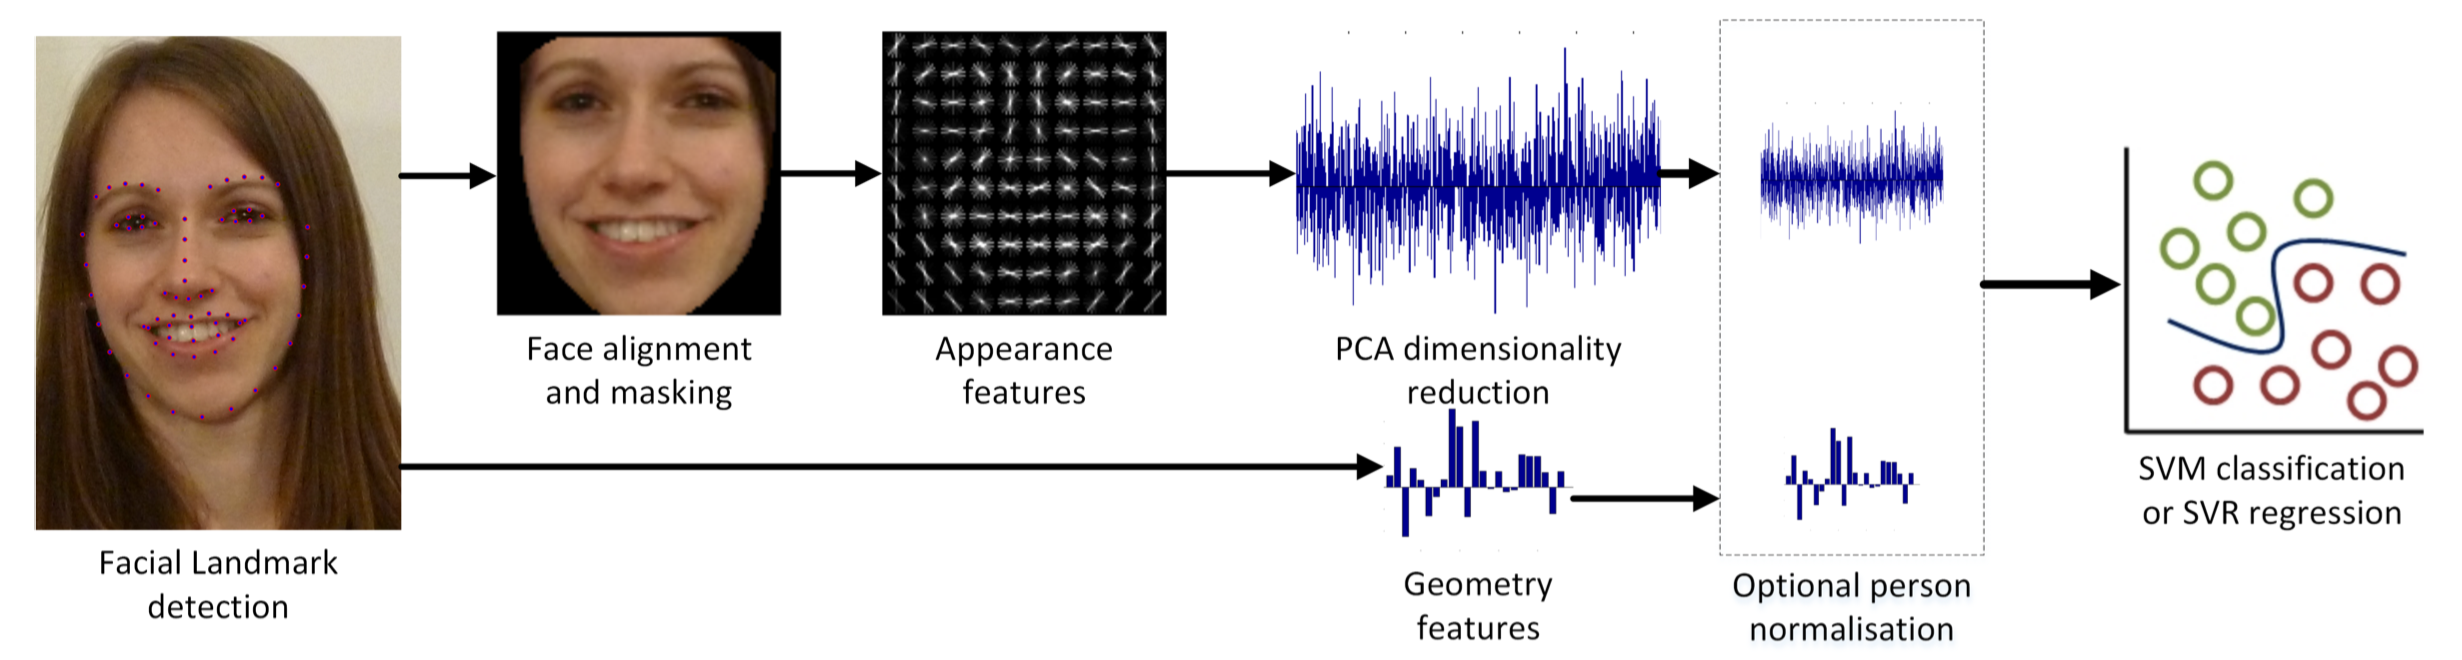
\includegraphics[width=1\textwidth]{AU_pipeline}
	\caption{AU detection and intensity pipeline \cite{Baltru2015}.}
	\label{fig:AU_pipeline}
\end{figure}

\subsection{Training Datasets}
%todo: this part might not be necessary here? I could expand a lot on it in the experiments section
There are four main dataset used for training the Action Unit detection system: DISFA \cite{DISFA}, BP4D-Spontaneous \cite{BP4D-Spontaneous}, SEMAINE \cite{SEMAINE} and CK+ \cite{CK+}. These four datasets consist of videos of people subject to emotion inducing tasks.

The \textbf{BP4D} database of spontaneous facial expressions includes videos of 41 participants (23 women and 18 men, 21 for training and 20 for validating). The age ranged from 18 to 29; 11 were Asian, 6 African-American, 4 Hispanic, and 20 Euro-American. \\
Emotion inducing techniques were used to elicit an emotional response. Frame-level ground-truth for facial actions was obtained by using the Facial Action Coding System annotations, performed by trained professionals. \\
Each participant in the database is associated with 8 tasks. For each task, there are both 3D and 2D videos and the metadata include annotations for 11 AUs for occurrence and 5 AUs for intensities.

\textbf{DISFA} (Denver Intensity of Spontaneuos Facial Action) Database is a non posed facial expression database for automatic action unit detection. It contains videos of 27 participants (12 female, 15 males; 14 used for training and 13 for validation). It includes 4 minute-long videos of spontaneous facial expression, resulting in 130k frames annotated for 12 AUs (Fig. \ref{fig:DISFA_AU}), comprehensive of AUs intensity on a 0 to 5 scale.

\begin{figure}[H]
	\centering
	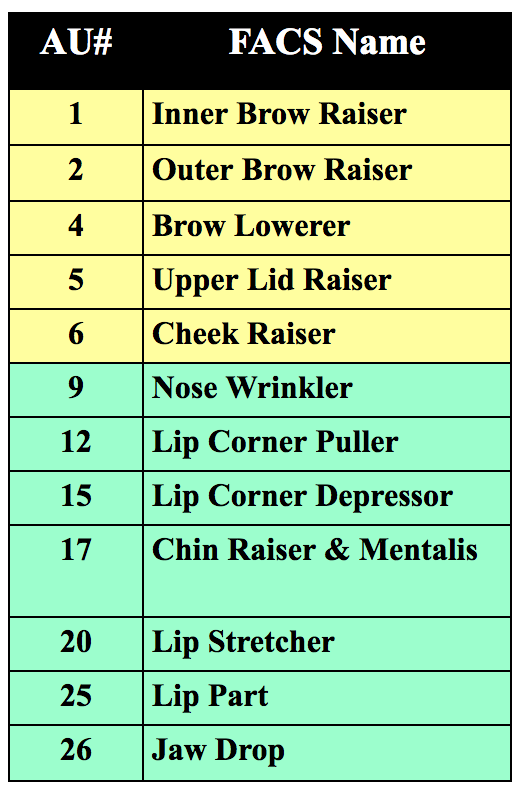
\includegraphics[width=0.5\textwidth]{DISFA_AU}
	\caption{AUs coded in the DISFA database \cite{DISFA_AU}.}
	\label{fig:DISFA_AU}
\end{figure}

The FACS annotated \textbf{SEMAINE} subset contains recordings of 31 subjects (15 for training and 16 for validation). It consists of one minute long recordings, leading to 93k frames labeled for 5 AU occurrences.

The \textbf{Cohn-Kanade} AU-Coded Facial Expression Database is utilized for research in facial image analysis. \\
CK+, includes both posed and non-posed (spontaneous) expressions and additional types of metadata. Each posed expression is completely FACS coded, and emotion labels are part of the metadata. \\
CK+ also provides baseline results for facial feature tracking, action unit and emotion recognition.

BP4D, SEMAINE and DISFA have three AUs in common (2, 12, and 17). \\
SEMAINE and DISFA share AUs 2, 12, 17, 25. \\
BP4D and DISFA share AUs 1, 2, 4, 6, 12, 15, 17. \\
This allows for cross-dataset training.

By training on these dataset is possible to detect the following AUs (\ref{fig:all_AUs}):

\begin{figure}[H]
	\centering
	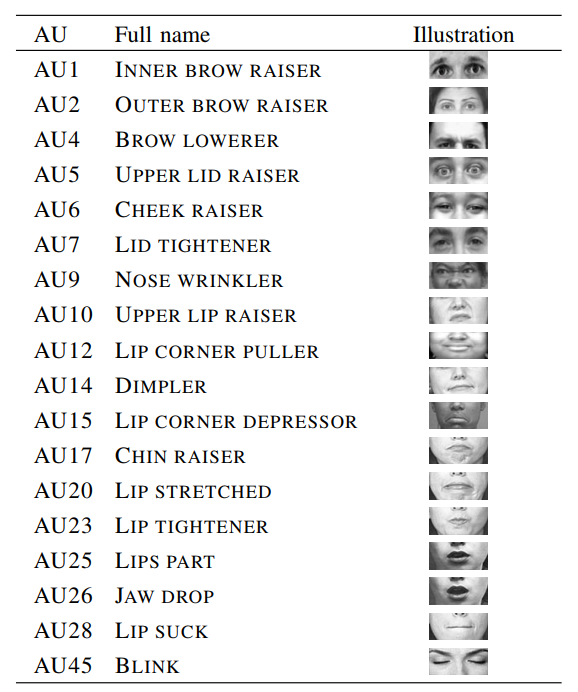
\includegraphics[width=0.85\textwidth]{all_aus}
	\caption{List of available AUs for prediction \cite{Baltru2018}.}
	\label{fig:all_AUs}
\end{figure}

\subsection{Feature Extraction}
There are two types of features that are used: appearance (Histogram of Oriented Gradients) and geometry (shape parameters and landmark locations) ones. To extract those features it's required to track certain landmarks on the face, and then continue this process by performing face alignment.

\subsubsection{Face Tracking}
%TODO: rewrite
Face tacking is done by utilizing Constrained Local Neural Field (CLNF) facial landmark detector and tracker, backed up by a structural SVM for facial detection \cite{Baltru2013}.
CLNF is a specific case of Constrained Local Model (CLM), that differs from the original by utilizing more advanced local detectors and a different optimization function.

The Constrained Local Model can be described by the following parameters: \\
$p = [s, \mathbf{R}, \mathbf{p}, \mathbf{t}]$.
\begin{itemize}[noitemsep, topsep = -5pt]
	\item \textit{s} is the scale factor.
	\item \textbf{R} is the object rotation.
	\item \textbf{t} is the 2D translation.
	\item \textbf{p} describes the shape of a vector of non rigid variations.
\end{itemize}

These parameters can be modified to compute different versions of the model. The resulting point distribution model is:

\begin{equation} \label{eq:pdm}
	x_i = s \cdot \mathbf{R}(\overline{x_i} + \phi_i \mathbf{p}) + \mathbf{t}
\end{equation}

Where $x_i$ is the location of the i\textit{th} feature point in an image, $\overline{x_i}$ is the mean of the i\textit{th} element of the PDM, and $\phi_i$ is the i\textit{th} eigenvector that describes the variation of the feature point.

In the Constrained Local Model we use the parameters from face detection to estimate the maximum a posteriori probability \textit{p} of the face model.

\subsubsection{Alignment and Masking}
For the extracted face to be correctly analyzed, there needs to be a mapping to a common reference frame, and the changes resulting from scaling and in plane rotation needs to be removed. 

In order to achieve this, a similarity transform from the currently detected landmarks to a representation of frontal landmarks from a neutral expression (projection of mean shape from a 3D PDM) is utilized. \\
The similarity transform is done with Procrustes superimposition that minimizes the mean square error between aligned pixels \cite{Baltru2013}.\\
The result is a $112 \times 112$ pixel image of the face with 45 pixel interpupillary distance (Fig \ref{fig:alignment_masking}). 

To reduce the weight of significant facial expressions (mouth opening, brow raises etc.) on the similarity transform, only the most stable facial landmarks must be used. \\
%TODO: non mi piace
In order to determine those points, the most stable CLNF detected landmarks on the CK+ dataset \cite{CK+} are examined.

\begin{figure}[H]
	\centering
	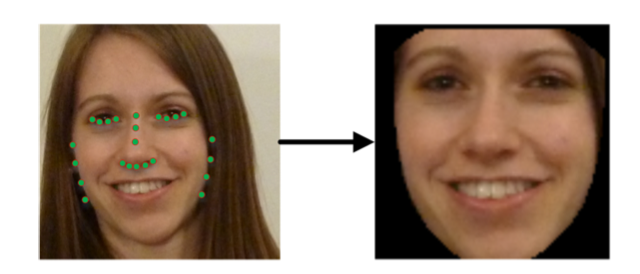
\includegraphics[width=0.75\textwidth]{alignment_masking}
	\caption{Stable points used for alignment to a common reference frame, followed by masking \cite{Baltru2015}.}
	\label{fig:alignment_masking}
\end{figure}

Masking, performed using a convex hull surrounding the feature points, is done to remove informations from the image that do not regard the face.

\subsubsection{Appearance Features}
After the face is aligned to a $112 \times 112$ image it's time to extract the appearance features. \\
To get the appearance features, $12 \times 12$ block of 31 dimensional Histogram of Oriented Gradients (HOG) are extracted, giving a 4464 dimensional vector characterizing the face. The implementation for HoG comes from dlib \cite{dlib}.

Once the feature vector is obtained, the next step is to reduce it's dimensionality. In order to do that Principal Component Analysis (PCA) is applied. \\
To generalize the dimensionality reduction, the training was performed on the FERA 2015 \cite{FERA15}, CK+ \cite{CK+}, DISFA \cite{DISFA}, AVEC 2011 \cite{AVEC11} and FERA 2011 \cite{FERA11} datasets. \\
By using PCA while sub-sampling from peak and neutral expressions and keeping 95\% of explained variability, the feature vector becomes of 1379 dimensions.

\subsubsection{Geometry Features}
%TODO: CHECK CLNF STUFF
The geometry features are obtained trough the CE-CLM models, and consist of non-rigid shape parameters and landmarks locations ($p$ and $ \phi_i p$ in equation \ref{eq:pdm}). this results in a 227 dimensional vector representing geometry features.\\
Summed to the appearance features, this leads to a 1606 dimensional vector that defines the appearance of the face.

\subsubsection{Neutral Expression Extraction}
To extract some of the facial expression is very important to have a neutral starting expression. There are personal differences on how we appear while in a neutral resting state, such as people looking naturally more cheerful or sad then others \cite{normexpr}. To address this issue there needs to be a person specific calibration, done by adjusting for neutral expressions \cite{Baltru2013}.

Neutral expression adjustments are done by computing the median value of the face descriptors in a video, leading to a neutral expression descriptor. This works assuming that in a video most of the frames will contain a neutral expression, and this should hold true especially for real life situations where most of the time the interactions are performed with a neutral expression \cite{NatAffData}.

Once the neutral descriptor is computed, it is subtracted from the feature descriptor, giving normalized features. 
%To help with the ease of computing the median, a histogram is kept for each element in the feature vector.

\subsubsection{Classification and Regression}
The next step is to extract Action Units from each frame of the video. Both intensity and presence are extracted.

Action Units detection is performed through Support Vector Machines (SVM), and Action Unit intensity using Support Vector Regression (SVR), both using the liblinear implementation \cite{liblinear}. In both cases a linear kernel is utilized, as more complex kernels had no effect on performances and were quite slower to train.  

Since the AU occurrences are not balanced by nature (for example AU28, blinking, is not very frequent if we analyze each frame of a video), it's highly important to balance the training data. To do this it was needed to undersample the negative AU samples from training data, thus getting to an equal number of positive and negative samples.

\clearpage

\section{Deception Detection} \label{dec_det}
%TODO: rewrite, tentative
In this step we feed the extracted action units from the videos to an SVM for classification.
We use an SVM because after a lot of testing with different techniques that was the one that performed the best compared to others. 

%todo: come prendiamo i dati, cosa facciamo... 
\subsection{Data pre-processing}
Before feeding the videos to the SVM for Action Units extraction we had to make sure the videos were in good enough condition to be processed. That is not given since all this videos come from real life trials and the recording conditions are not optimal.

Being in an acceptable condition means that the face should be clearly visible, and the video has to have the specific person visible and talking in at least \textit{most} of the video, and no other people on it, so to avoid training on different subjects of which we are not sure if they are lying or telling the truth.

As a consequence many videos had to be cut, trimmed or discarded to reach an acceptable level.

After extracting Action Units intensity and presence from our dataset of videos (\ref{rldb}) we put the data in a \textit{csv} format to be able to process them and pass them to the SVM. 

The data are divided for both AUs intensity, ranging from $0$ to $5$, and AU presence, having the boolean value of either $0$ or $1$ if the AU was missing or present in the specific frame of the video.

\begin{figure}[H]
	\centering
	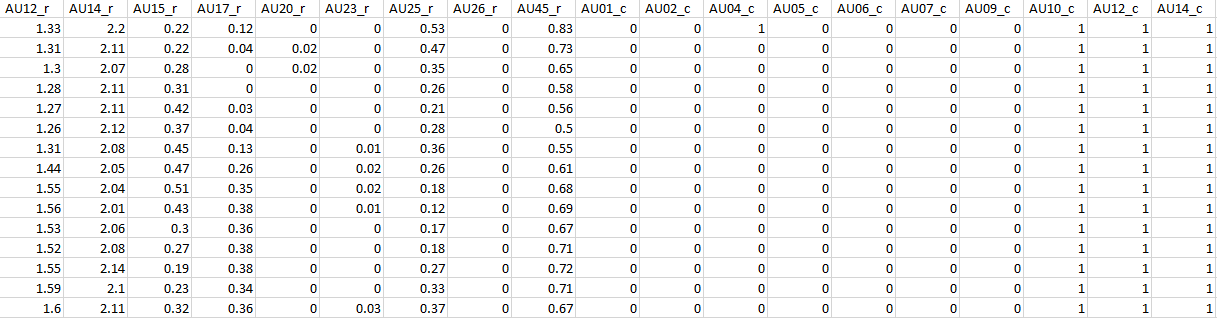
\includegraphics[width=1\textwidth]{dataset_csv}
	\caption{Example of input data in csv format.}
	\label{fig:dataset_csv}
\end{figure}

The next step is to remove all the rows that have both no intensity and no presence for AUs, since those rows are most likely errors from the extraction, deriving from the poor quality of the videos, or from the face not being recognized in some frames.

%todo: forse non e' utile qui ma in generale lo devo dire
We organized the data in three sets, one concerning only AUs intensity, one with only AUs presence, and another one where we merged the previous ones together, in order to better analyze the data and understand it's structure.

\subsection{SVM}
%todo: svm personalizzato a quello che ho fatto

After pre-processing the data we use the train set to train a sigmoid %lo metto o solo svm?
SVM, and then we utilize the trained model to evaluate on the test set and compare the results with the labels present on the test set.

Generally, each of \textit{n} frames is converted in a vector of length 36, where 17 variables represent the intensity and 18 variables represent the presence of Action Units. The last variable is the class label.

%todo: check better way to formalize this
So a given training input \textbf{AU} for our SVM, \textbf{AU} is a $36 \times n$ matrix composed of $AUI_i$ and $AUP_i$, where $AUI_i$ represents the intensity for action units in row \textit{i} and $AUP_i$ is the action units presence for row \textit{i}. 

These observations belong to two classes, truthful and deceptive, represented by a label \textbf{Y} = $\{y_1 \dots y_n\}$, where $y = \{0,1\}$ depending on whether the frame belongs to a deceptive or truthful observation.

\begin{equation}
	\mathbf{AU} = (AUI_i + AUP_i, y_i)
\end{equation}

An input vector $au^*$ for the test set, this time of length 35, is formed the same way but without having a class label.

\begin{equation}
	\mathbf{au^*} = (AUI^*_1 + AUP^*_1, \dots, AUI^*_{35} + AUP^*_{35})^T
\end{equation}

The goal of our SVM classifier is to correctly classify the test observation based on the training done by using the data in the train set.

%todo: recheck
Suppose we are using a \textit{linear} SVM classifier. We would need to figure out weather a point lies on one side or the other of an hyperplane, and we would look at this kind of equations to classify a test observation $au^*$ based on the sign of $f(au^*)$:

\begin{equation} 
	f(au^*) = \beta_0 + \beta_1 au^*_{1} + \beta_2 au^*_{2} + \dots + \beta_{35} au^*_{35}
\end{equation}

if $f(au^*)$ is positive, then we would assign the test observation to class 1, and if it is negative, we would assign it to class 0.

Of course there are two things we need to consider:
- we need to keep the margin M of the hyperplane in consideration
- the relationship between features is not linear so we could need to enlarge the feature space

For the Support Vector Machine we enlarge the feature space using kernel functions \ref{kernel}

%figure with SVM with AUs divided by a line (or whatever)

%todo: equations from ML chapter rewritten using X





\chapter{Experiments}
%TODO: obviously rewrite this
In this section I will describe the stack used for this thesis and the experiments done to achieve our results: I will start by reviewing the configurations and libraries utilized (par. \ref{bb}), the database used to acquire training and test set (Par. \ref{rldb}), all the analysis done on the data (par. \ref{data_an}), and finally the results (par. \ref{res}).

\section{Building Blocks} \label{bb}
To realize this work we used the following tools and libraries:
\begin{itemize}
	\item OpenFace: the library to train the models for face detection, landmark detection, feature extraction and action unit recognition.
	\item R + R-Studio: the environment where I implemented the code, with some important libraries, such as:
	\begin{itemize}
		\item e1071: library for SVM classification (implementation of libsvm).
		\item Random Forest: library to perform Random Forest and calculate variable importance.
		\item Corrplot: library for calculating and visualizing correlations.
	\end{itemize}
\end{itemize}

The experiments were conducted on two systems, Windows and Mac OS, with the following specs:\\
The windows machine has 8GB of RAM, i5 processor, and 4096MB ATI AMD Radeon R9. \\
The Mac has 4gb RAM, i5 processor, and an intel integrated GPU.\\
SVM training took about one hour on both machines.

\clearpage

%TODO: SHORT review (table pherhaps) of face db, maybe not in this section
\section{Real Life Trial Database} \label{rldb}
This section is about the database we used to perform our experiments: it comes from the work done for the paper "Deception Detection using Real-life Trial Data" \cite{Perez-Rosas:2015:DDU:2818346.2820758}.

\begin{figure}[H]
	\centering
	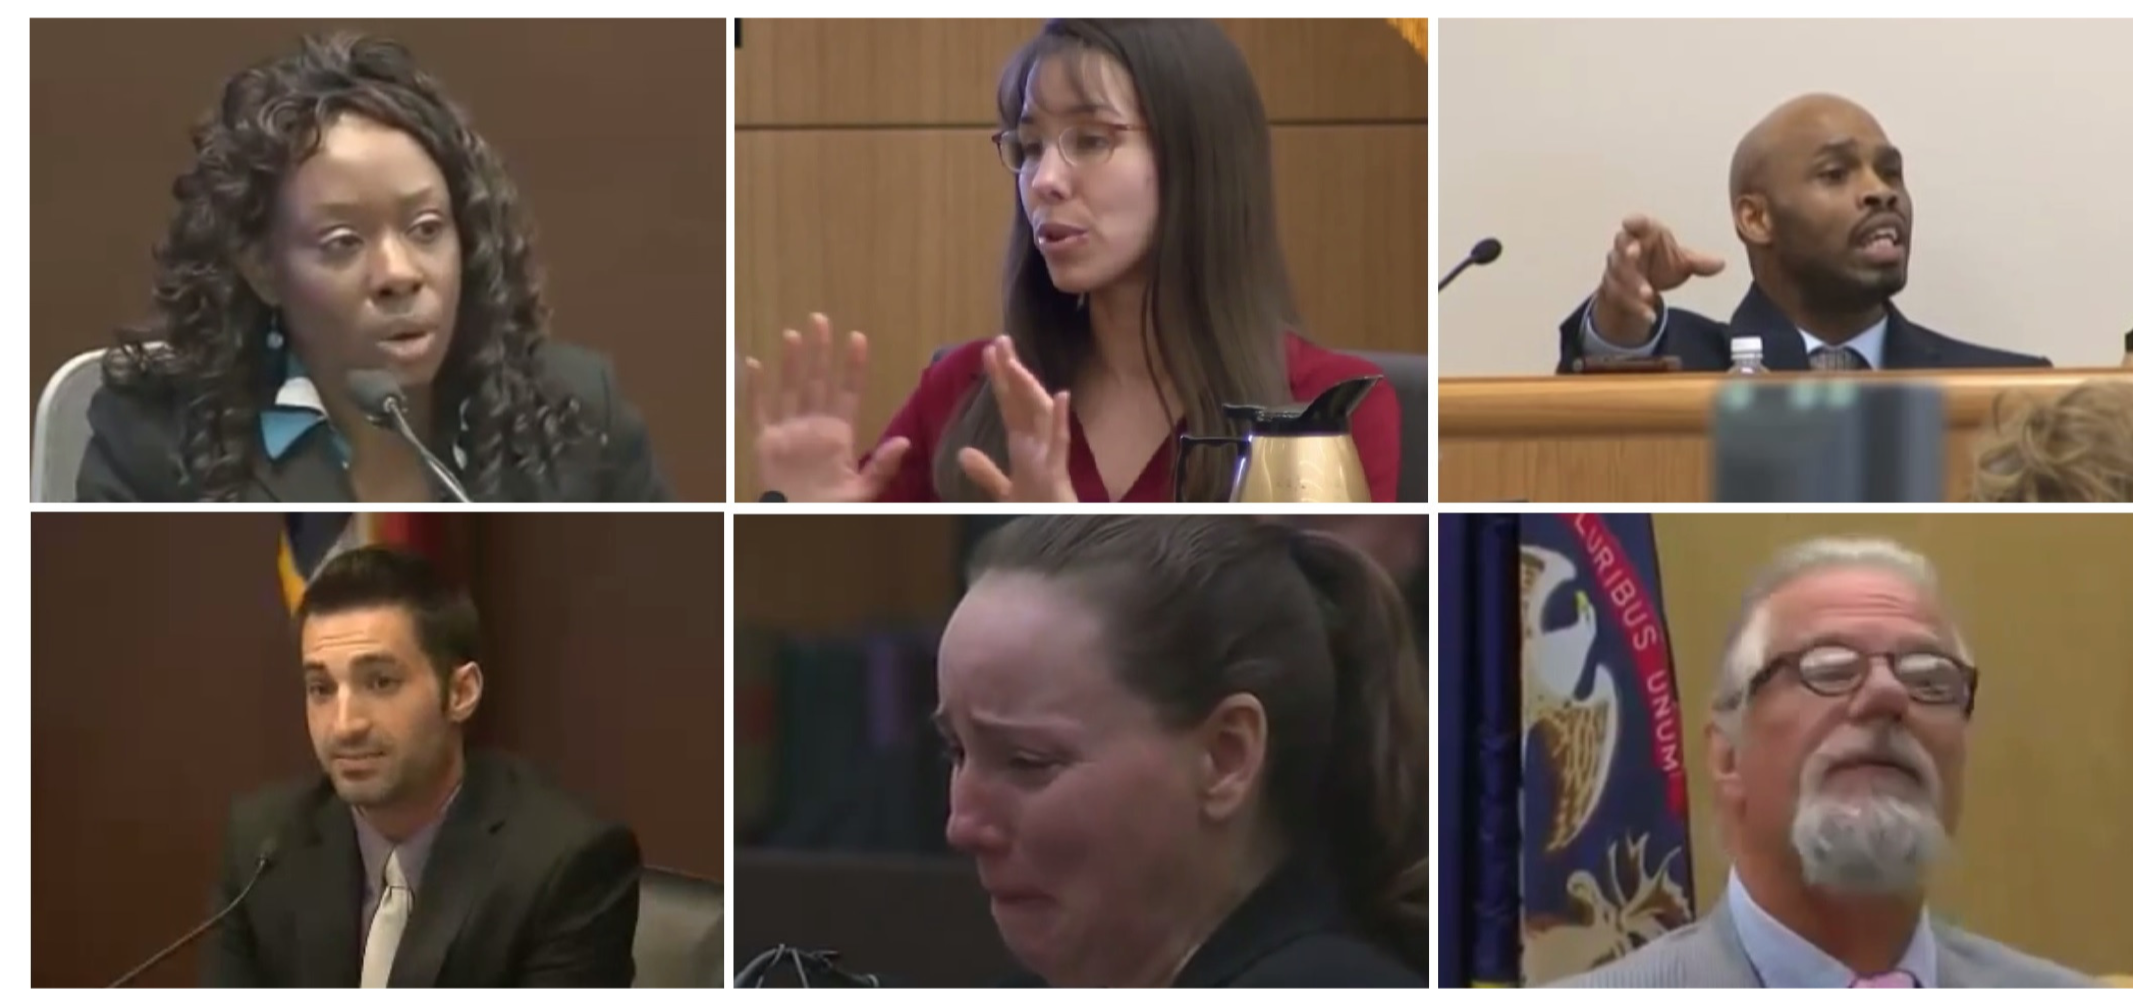
\includegraphics[width=1\textwidth]{trial_images}
	\caption{Examples of images from the dataset videos. \cite{Perez-Rosas:2015:DDU:2818346.2820758}.}
	\label{fig:trial_images}
\end{figure}


The dataset is gathered from real-life trial videos available on YouTube and other public websites. The dataset also contains statements made by exonerees after exoneration, and some statements from defendants during crime-related TV episodes.

The first step to collecting the dataset was to identify public multimedia sources where the recordings of the trials were available, and deceptive and truthful behavior could be observed and verified.\\
The videos are of trial recordings where the defendant or witness in the video can be clearly identified, the face is visible enough during most of the clip duration, and the visual quality should be good enough to accurately see the facial expressions (Fig. \ref{fig:trial_images}).\\
There are three outcomes for the trials that were considered to label the videos as deceptive or truthful: guilty, non-guilty, and exoneration. \\
For the guilty verdicts the deceptive clips are taken from the defendant in the trial, while the truthful clips are gathered from the witnesses. There are also instances where the deceptive videos are of suspects denying a committed crime, and truthful ones are from the same person answering questions that where verified by the police as truthful.

In regards to the witnesses, if the testimony is verified by a police officer they are labeled as true. \\ 
Testimonies that help the guilty party are labeled as false. Exoneration (reversal of the sentence) testimonies are regarded as truthful.

The original dataset consists of 121 videos, 61 of which are deceptive and 60 truthful. \\
The average length of the videos is 28.0 seconds. The average video length for deceptive videos is 27.7 seconds, while the one for truthful videos is 28.3 seconds. \\
The data consists of 58 total subject, 22 females and 36 males, with ages between 16 and 60 years.

This dataset was annotated following the MUMIN coding scheme for hand movement and facial displays. While annotating, the annotators were able to chose only one label per gesture, for every clip.

Fig. \ref{fig:rldb_distrib} shows the frequency counts associated with the gestures considered during the annotation.

\begin{figure}[H]
	\centering
	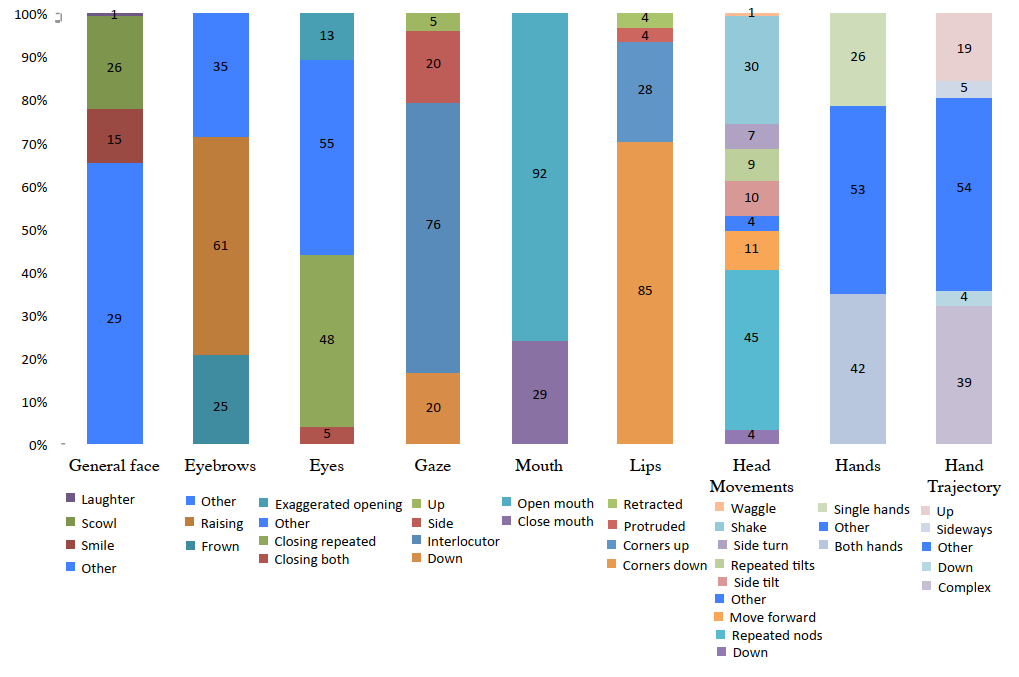
\includegraphics[width=1\textwidth]{rldb_distrib}
	%todo: change caption
	\caption{Examples of images from the dataset videos. \cite{Perez-Rosas:2015:DDU:2818346.2820758}.}
	\label{fig:rldb_distrib}
\end{figure}

%TODO: modification made by me to the DB 
%TODO: rewrite tentative atm

We modified this database in the following way:
\begin{itemize}
	\item We cut or removed videos where the where the face was covered, hidden or in very difficult to see.
	\item We also cut parts of video that had multiple subjects in the scene because Action Unit extraction works on one person only.
	\item Since it is necessary to see the person to perform AU extraction, we also avoided some videos in which the subject was not visible while talking (the interlocutor was shown).
\end{itemize}

With deceptive videos going from \#1 to \#61 and truthful videos going from \#1 to \#60 we cut and removed the following videos from the original dataset, since they showed signs of the problems just described:

\begin{itemize}
	\item \textbf{Deceptive}:
	\begin{itemize}
		\item CUT: Video numbers 46, 47, 48, 49, 52, 54, 56.
		\item REMOVED: Video numbers 50, 53,  55.
	\end{itemize}
	\item \textbf{Truthful}:
	\begin{itemize}
		\item CUT: Video number 7, 28, 43.
		\item REMOVED: Video numbers 12, 31. 
	\end{itemize}
\end{itemize}


We also performed a division of subjects in the training and test set "by hand", splitting data to around 75\% for the training set and 25\% for the test set, to train the classifiers in a way that it wouldn't adapt the specific people since there are many videos with the same subject. In fact, the same person never appears both in the training and in the test set.

The training set consists of 72451 observations of 36 variables, and the test set is 14198 observations.
%todo: stats of db, #of frames ecc

\clearpage

\section{Data Analysis} \label{data_an}
In the following sections we describe the methods used to analyze the data and the machine learning techniques to classify them. \\
We start with comparing the occurrences for deceptive and truthful videos on the training set (par. \ref{data_comp}), then look at the correlation between variables (par. \ref{corr}), then we explain how we used GLM (par. \ref{GLM}), Random Forest (par. \ref{rf}) and Support Vector Machines (par. \ref{SVM})

\subsection{Data Comparison} \label{data_comp}
The first thing I did, after cleaning the data, was to compare the extracted deceptive (Fig \ref{fig:au_occ_dec}) and truthful (Fig. \ref{fig:au_occ_truth}) AUs occurrences (only for presence, not intensity) from the training set, which is shown in Fig. \ref{fig:au_occ_comp}.

\begin{figure}[H]
	\centering
	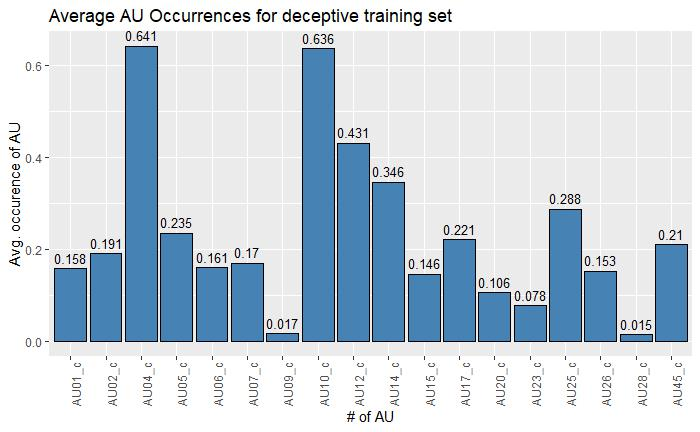
\includegraphics[width=1\textwidth]{images/au_occ_dec}
	\caption{Average AU Occurrences for the deceptive training set.}
	\label{fig:au_occ_dec}
\end{figure}

\clearpage

\begin{figure}[H]
	\centering
	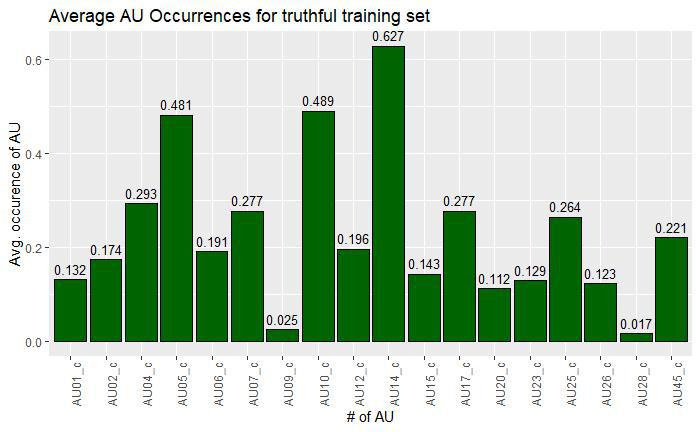
\includegraphics[width=1\textwidth]{images/au_occ_truth}
	\caption{Average AU Occurrences for the truthful training set.}
	\label{fig:au_occ_truth}
\end{figure}

\begin{figure}[H]
	\centering
	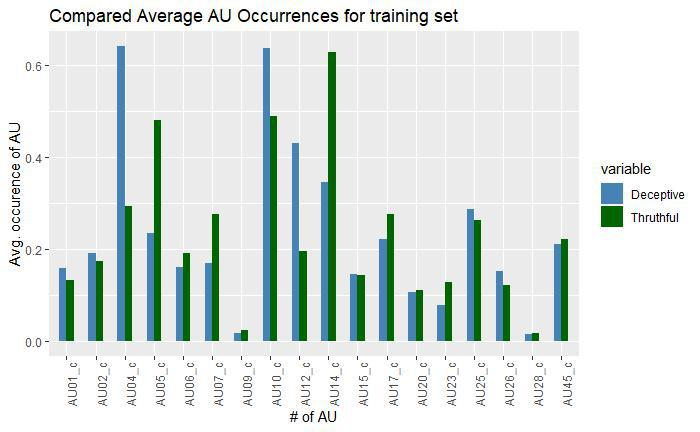
\includegraphics[width=1\textwidth]{images/au_occ_comp}
	\caption{Comparison of AU Occurrences for the training set.}
	\label{fig:au_occ_comp}
\end{figure}

This comparison shows interesting differences between truthful and deceptive occurrences for AU04 (Brow Lowerer), AU05 (Upper Lid Raiser), AU10 (Upper Lip Raiser), AU12 (Lip Corner Puller) and AU14 (Dimpler). %"suggesting there could be a pattern"?

\subsection{Correlation} \label{corr}
Variables correlation is shown in figure \ref{fig:correlation_matrix}. When the AUs label ends with "\_r" it indicate intensity and "\_c" means presence.

\begin{figure}[H]
	\centering
	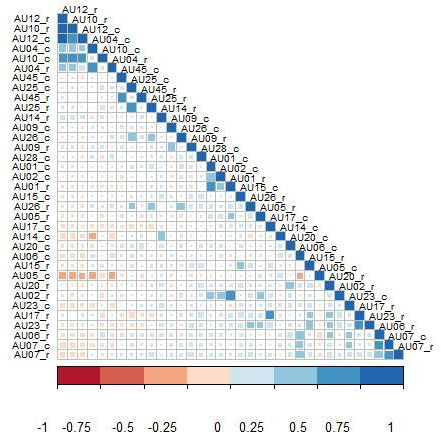
\includegraphics[width=1\textwidth]{images/correlation_matrix}
	\caption{Correlation between variables for both presence and intensity in the training set.}
	\label{fig:correlation_matrix}
\end{figure}

%todo: positive corr with, neg corr with...
which shows some obvious correlations between presence and intensity of the same AU, and significant correlation between AU10\_r, AU12\_r, AU12\_c, AU07\_r, AU17\_r, AU06\_r, AU04\_c, AU02\_r, AU01\_r, AU25\_r, AU45\_c.

\clearpage

\subsection{GLM} \label{GLM}
Another quick experiment I made was with the Generalized Linear Model in R, which translates into Logistic Regression (Par. \ref{logreg}), at least to have an idea of the resulting p-values, as seen in fig. \ref{fig:pval}:

\begin{figure}[H]
	\centering
	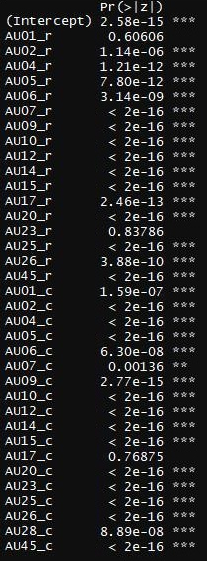
\includegraphics[width=0.5\textwidth]{images/pval}
	\caption{p-values from GLM for each AU (intensity and presence).}
	\label{fig:pval}
\end{figure}

As we can see AU01\_r (Inner Brow Raiser), AU23\_r (Lip Tightener), and AU17\_c (Chin Raiser) are not significant and that's an indication that we could remove them from the dataset.

%todo: should i say this?
The results for classifying data with GLM is 54.86\% accuracy on the test set, which is a little better than chance but not great. 

\clearpage

\subsection{Random Forest} \label{rf}
I've decided to use Random Forest (par. \ref{random_forest}) to estimate variable importance, shown in fig. \ref{fig:varimp}.

\begin{figure}[H]
	\centering
	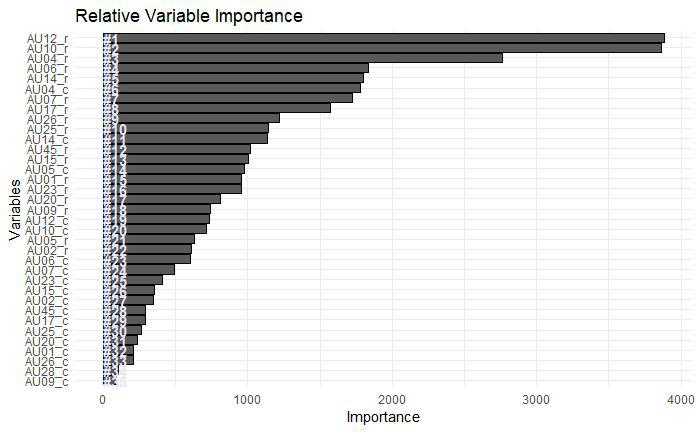
\includegraphics[width=1\textwidth]{images/varimp}
	\caption{Variable Importance extracted from classifying data with Random Forest.}
	\label{fig:varimp}
\end{figure}

The number of grown trees are 200 as going further did not increase the prediction accuracy at all.

Fig. \ref{fig:varimp} shows that the intensity of AUs 04, 06, 07, 10, 12 and 14 are the most significant, while the sole presence of an AU is not particularly significant, beside for AUs 04, 05 and 14.

As we can see AUs that have low p-values in GLM have also low importance in Random Forest.

Classifying with Random Forest gave me 58,42\% accuracy on the test set, which is better than GLM but it is still not good enough to be significant.

\clearpage

\subsection{SVM} \label{SVM}
To approach classification with an SVM we tried both a linear and radial kernel.

%todo: specify how much is C and gamma
The cost $c$ and $\gamma$ parameter were found using a tuning function that perform a grid search over the combinations of cost and gamma for both kind of kernels.

The results for classifying with a linear kernel are 66,34\% accuracy on the test set, which is a good starting result, while a radial kernel performs worse at around 61\% accuracy.


\chapter{Results}
Results obtained

\section{Tests and Results} 

\chapter{Conclusions}
%todo: WRITE THEM
Conclusion

%todo: useful shit?
FUTUREU USE - app per telefono video -> result

 Since the videos in our database were mostly collected from YouTube, certain uncontrollable factors add to the difficulty of their analysis. \\
These totally unconstrained and spontaneous videos are subject to temporal variations in illumination, head pose and facial occlusion.

\section{Final Considerations}
In this thesis we presented a way to discriminate between lies and truths, based on AUs extraction and SVM classification.
%todo: privacy concerns?



\section{Future Work}
Some possible developments to be applied to this thesis are:
\begin{itemize}
	\item One of the difficulties of this kind of studies is the lack of a big dataset for high stake deception. It would be beneficial to gather such dataset to improve the results, bettering also the quality of the images.
	\item Extend AUs extraction to more than one person in the scene. It would be interesting to consider direct interaction with questions and responses. 
	\item Using temporal information for each video to capture the beginning and the end of the interaction. The lie does not necessarely appear in \textit{all} the video, but probably just at some point, even though the majority of the statements are either deceptive or truthful. We were thinking about LSTM to observe the temporality.
	\item More modules to consider other than the face. We could consider the body, and analyze the voice and speech patterns to extract information from the subject.
\end{itemize}

\backmatter

\printbibliography

\listoffigures

\cleardoublepage

\end{document}
